\documentclass[a4paper]{article}
\usepackage{a4wide,amssymb,epsfig,latexsym,multicol,array,hhline,fancyhdr}
\usepackage{vntex}
\usepackage{amsmath}
\usepackage{lastpage}
\usepackage[lined,boxed,commentsnumbered]{algorithm2e}
\usepackage{enumerate}
\usepackage{color}
\usepackage{graphicx}							% Standard graphics package
\usepackage{array}
\usepackage{tabularx, caption}
\usepackage{multirow}
\usepackage{multicol}
\usepackage{rotating}
\usepackage{graphics}
\usepackage{geometry}
\usepackage{setspace}
\usepackage{epsfig}
\usepackage{tikz}
\usepackage{booktabs}
%\usepackage[vietnamese]{babel}
\usetikzlibrary{arrows,snakes,backgrounds}
\usepackage{hyperref}
\hypersetup{urlcolor=blue,linkcolor=black,citecolor=black,colorlinks=true} 
%\usepackage{pstcol} 								% PSTricks with the standard color package

\newtheorem{theorem}{{\bf Định lý}}

\newtheorem{property}{{\bf Property}}
\newtheorem{proposition}{{\bf Proposition}}
\newtheorem{corollary}[proposition]{{\bf Corollary}}
\newtheorem{lemma}[proposition]{{\bf Lemma}}

\AtBeginDocument{\renewcommand*\contentsname{Mục lục}}
\AtBeginDocument{\renewcommand*\refname{Tài liệu tham khảo}}
%\usepackage{fancyhdr}
\setlength{\headheight}{40pt}
\pagestyle{fancy}
\fancyhead{} % clear all header fields
\fancyhead[L]{
 \begin{tabular}{rl}
    \begin{picture}(25,15)(0,0)
    \put(0,-8){\includegraphics[width=8mm, height=8mm]{hcmut.png}}
    %\put(0,-8){\epsfig{width=10mm,figure=hcmut.eps}}
   \end{picture}&
	%\includegraphics[width=8mm, height=8mm]{hcmut.png} & %
	\begin{tabular}{l}
		\textbf{\bf \ttfamily TRƯỜNG ĐẠI HỌC BÁCH KHOA - ĐHQG-HCM}\\
		\textbf{\bf \ttfamily KHOA KHOA HỌC VÀ KỸ THUẬT MÁY TÍNH}
	\end{tabular} 	
 \end{tabular}
}
\fancyhead[R]{
	\begin{tabular}{l}
		\tiny \bf \\
		\tiny \bf 
	\end{tabular}  }
\fancyfoot{} % clear all footer fields
\fancyfoot[L]{\scriptsize \ttfamily Bài tập lớn môn Mô hình hóa toán học - HK 231 2023 - 2024}
\fancyfoot[R]{\scriptsize \ttfamily Page {\thepage}/\pageref{LastPage}}
\renewcommand{\headrulewidth}{0.3pt}
\renewcommand{\footrulewidth}{0.3pt}


%%%
\setcounter{secnumdepth}{4}
\setcounter{tocdepth}{3}
\makeatletter
\newcounter {subsubsubsection}[subsubsection]
\renewcommand\thesubsubsubsection{\thesubsubsection .\@alph\c@subsubsubsection}
\newcommand\subsubsubsection{\@startsection{subsubsubsection}{4}{\z@}%
                                     {-3.25ex\@plus -1ex \@minus -.2ex}%
                                     {1.5ex \@plus .2ex}%
                                     {\normalfont\normalsize\bfseries}}
\newcommand*\l@subsubsubsection{\@dottedtocline{3}{10.0em}{4.1em}}
\newcommand*{\subsubsubsectionmark}[1]{}
\makeatother


\begin{document}

\begin{titlepage}
\begin{center}
ĐẠI HỌC QUỐC GIA THÀNH PHỐ HỒ CHÍ MINH \\
TRƯỜNG ĐẠI HỌC BÁCH KHOA \\
\textbf{KHOA KHOA HỌC VÀ KỸ THUẬT MÁY TÍNH}
\end{center}

\vspace{1cm}

\begin{figure}[h!]
\begin{center}
\includegraphics[width=3cm]{hcmut.png}
\end{center}
\end{figure}

\vspace{1cm}


\begin{center}
\begin{tabular}{c}
\multicolumn{1}{l}{\textbf{{\Large MÔ HÌNH HÓA TOÁN HỌC (CO2011)}}}\\
~~\\
\hline
\\
\multicolumn{1}{l}{\textbf{{\Large Bài tập lớn}}}\\
\\
\textbf{{\Huge QUY HOẠCH NGẪU NHIÊN}}\\
\\
\textbf{{\Huge VÀ CÁC ỨNG DỤNG}}\\
\\
\hline
\end{tabular}
\end{center}

\vspace{2cm}

\begin{table}[h]
\begin{tabular}{rrl}
\hspace{5 cm} & GVHD: & Mai Xuân Toàn\\
& Students: & Hồ Minh Hưng - 2211361 - Nhóm trưởng \\
& &  Võ Quốc Huy - 2211303 \\
& &  Mai Hoàng Huynh - 2211314 \\
& &  Phạm Duy Hưng - 2211379 \\
& &  Phạm Hoan Huy - 2211264 \\
\end{tabular}
\end{table}

\begin{center}
{\footnotesize TP.HỒ CHÍ MINH, THÁNG 12/2023}
\end{center}
\end{titlepage}


%\thispagestyle{empty}

\newpage
\tableofcontents
\newpage


%%%%%%%%%%%%%%%%%%%%%%%%%%%%%%%%%
\section{Giới thiệu chung về Quy hoạch và tối ưu hóa ngẫu nhiên}
    \subsection{Quy hoạch là gì? Quy hoạch ngẫu nhiên là gì? Tính không chắc chắn?}
        \begin{itemize}
            \item \textbf{Tối ưu hóa toán học} là lĩnh vực về đưa ra quyết định, thường sử dụng các phương pháp toán học.
            \item \textbf{Quy hoạch ngẫu nhiên} (Stochastic Programming - SP) là lĩnh vực về việc đưa ra quyết định trong các trường hợp \textit{không chắc chắn}.
            \\Có thể xem nó như là `Quy hoạch (Tối ưu hóa) toán học với các tham số \textit{ngẫu nhiên}'.
            \item \textit{Quy hoạch tuyến tính ngẫu nhiên} là quy hoạch tuyến tính (tức là hàm mục tiêu của nó tuyến tính) mà trong đó một số thông tin về bài toán xem như chưa chắc chắn.
        \end{itemize}
    \subsection{Các nội dung cơ bản, Giả thiết - Mục tiêu}
        \textbf{Định nghĩa 1 (Quy hoạch tuyến tính (LP) với tham số ngẫu nhiên - SLP).} \\
            \hspace*{0.5cm} Một quy hoạch tuyến tính ngẫu nhiên là:
            \begin{displaymath}
            \text { Minimize } Z=g(\boldsymbol{x})=f(x)=c^T \cdot x, \quad \text { với } A x=b, \text { và } \quad T x \geq h
            \end{displaymath}
            \\
            \hspace*{0.5cm}với $\boldsymbol{x}=(x_{1}, x_{2},...,x_{n})$
            (các biến quyết định), \\
            \hspace*{0.5cm}ma trận thực $A$ và vector $b$ nhất định (cho các điều kiện ràng buộc),\\
            \hspace*{0.5cm}và các tham số ngẫu nhiên $T,h$ và 
            $T \: \boldsymbol{x} \geq h$ cho biết các ràng buộc về khả năng hoặc xác suất.
            \\
            \\
        \textbf{Ví dụ 1}. \textit{Xét tối ưu hóa sau}  
            \begin{displaymath}
                \text {Minimize z} = x_{1} + x_{2},
                \quad \text {với } x_{1} \geq 0,x_{2} \geq 0. \\
                \begin{cases}
                    \text{$\omega_{1} x_{1} + x_{2} \geq 7;$} \\
                    \text{$\omega_{2} x_{1} + x_{2} \geq 4.$} \\
                \end{cases}
            \end{displaymath}\\
            trong đó tham số $\omega_{1}$ và $\omega_{2}$ là biến đồng bộ (ngẫu nhiên), tuân theo phân phối sau:\\
            \hspace*{0.5cm} $Uniform(a,b)$, trong đó $\omega_{1} \sim Uniform(1,4)$ và $\omega_{2} \sim Uniform(1/3,1)$.\\
            \begin{itemize}
                \item Khi cả $\omega_{1} = \omega_{2} = 1$ thì hai điều kiện ràng buộc trở thành:\\
                $x_{1} + x_{2} = 4$ tạo nên đường màu đỏ, và $x_{1} + x_{2} = 7$ tạo nên đường nét đứt màu xanh,\\
                có thể thấy được vùng khả thi một cách đầy đủ thông qua mũi tên màu xanh lá. (Hình 1)\\
                \item \textbf{Vậy làm cách nào để giải bài toán này?}
                \begin{enumerate}
                    \item Phương pháp \textbf{wait - and - see (chờ và xem)}: Giả sử có thể chọn các biến quyết định
                    $x=[x_{1},x_{2}]$ \underline{sau khi quan sát} vector ngẫu nhiên $\omega=[\omega_{1},\omega_{2}]$?.
                    [biểu trưng một phần cho việc \textit{không chắc chắn về dữ liệu} của bài toán.]
                    Liệu có thể giải mà không cần phải chờ?
                    \begin{figure}[ht]
                        \centering
                        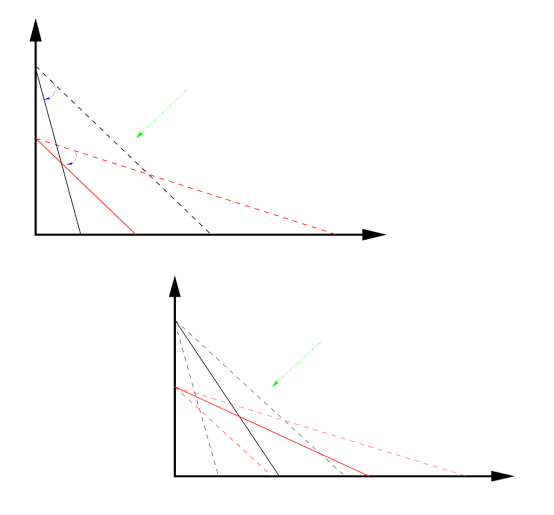
\includegraphics{plot.png}
                        \caption{Bài toán quy hoạch ngẫu nhiên đơn giản với hai biến quyết định.}
                    \end{figure}
                    \item Hoàn toàn có thể, giả sử cho $x=[x_{1}, x_{2}]$ \textbf{trước khi biết} giá trị của
                    $\omega=[\omega_{1},\omega_{2}]$? Ta cần chọn xem cần phải làm gì với việc \underline{không biết $\omega$} này.
                    Có hai cách như sau:\\(a) Đoán sự không chắc chắn, và (b) Các ràng buộc xác suất (xem lại Khái niệm 1).\\
                        \begin{enumerate}
                            \item \textbf{Đoán sự không chắc chắn:} Ta đoán thử một vài giá trị hợp lý cho $\omega$. Có ba giá trị như vậy, mỗi cái cho biết mức độ `rủi ro'
                                \begin{itemize}
                                    \item Unbiased: Chọn \underline{giá trị trung bình} cho mỗi tham số $\omega$.
                                    \item Pessimistic: Chọn giá trị trong \underline{trường hợp xấu nhất} cho $\omega$.
                                    \item Optimistic: Chọn giá trị trong \underline{trường hợp tốt nhất} cho $\omega$.
                                \end{itemize}
                        \end{enumerate}
                \end{enumerate}
                Chẳng hạn, sử dụng \textbf{phương pháp Unbiased}, xem lại ví dụ 1, phân phối
                đồng nhất Uniform(\textit{a,b}) có giá trị trung bình là $\frac{a+b}{2}$, vì vậy $\hat{\omega}=(\frac{5}{2}, \frac{2}{3})$. Quy hoạch lúc này trở thành
                \begin{displaymath}
                    \text {Minimize z} = x_{1} + x_{2}
                \end{displaymath}
                có giá trị tối ưu $z_{1} = \dfrac{50}{11}$ tại điểm $\hat{x}=(\hat{x_{1}}, \hat{x_{2}})=18/11,32/11$
                    \begin{displaymath}
                        \text{nếu giả sử}
                        \begin{cases}
                            \text{$\dfrac{5}{2}x_{1}+x_{2} \geq 7; \dfrac{2}{3}x_{1} + x_{2} \geq 4;$} \\
                            \text{$x_{1} \geq 0; x_{2} \geq 0$} \\
                        \end{cases}
                    \end{displaymath}
                Đối với \textbf{phương pháp Pessimistic}, $\hat{\omega}=[1, \dfrac{1}{3}]$
                \begin{displaymath}
                    \begin{cases}
                        \text{$\textbf{1}x_{1}+x_{2} \geq 7; \textbf{1/3}x_{1} + x_{2} \geq 4;$} \\
                        \text{$x_{1} \geq 0; x_{2} \geq 0$} \\
                    \end{cases}
                \end{displaymath}
                $\Longrightarrow z_{2}=7 \: \text{tại điểm} \: \hat{x}=(\hat{x_{1}},\hat{x_{2}})=(0,7)$\\
                Đối với \textbf{phương pháp Optimistic}, $\hat{\omega}=(4,1)$
                \begin{displaymath}
                    \begin{cases}
                        \text{$\textbf{4}x_{1}+x_{2} \geq 7; \textbf{1}x_{1} + x_{2} \geq 4;$} \\
                        \text{$x_{1} \geq 0; x_{2} \geq 0$} \\
                    \end{cases}
                \end{displaymath}
                $\Longrightarrow z_{3}=\dfrac{7}{4} \: \text{tại điểm} \: \hat{x}=(\hat{x_{1}},\hat{x_{2}})=(\dfrac{7}{4},0)$\\
            \end{itemize}

%%%%%%%%%%%%%%%%%%%%%%%%%%%%%%%%%
\section{Quy hoạch tuyến tính ngẫu nhiên một giai đoạn - Không phản hồi (One-Stage Stochastic linear programming - No recourse, 1-SLP)}

    \textbf{Định nghĩa 2 (1 - SLP).} \textit{Xét quy hoạch $LP(\alpha)$ sau được tham số hóa bởi vector ngẫu nhiên $\alpha$:}
    \begin{gather*}
        %\text{Minimize } Z=g(\boldsymbol{x})=f(x)=c^T \cdot x=\sum_{j=1}^{n} c_{j} x_{j} \\
        Minimize \; Z = g(\boldsymbol{x})=f(\boldsymbol{x})= c^T \cdot x=\sum_{j=1}^{n} c_{j} x_{j} \\
        \text{phụ thuộc} \quad A \, x=b, \quad \textit{(các ràng buộc chắc chắn)} \\
        \text{và} \quad T \, x \geq h, \quad \textit{(các ràng buộc ngẫu nhiên)}
    \end{gather*}
    với các giả thiết sau
    \begin{enumerate}
        \item Ma trận $T=T(\alpha)$ và vector $h=h(\alpha)$ biểu diễn sự không chắc chắn thông qua các ràng buộc ngẫu nhiên
            \begin{displaymath}
                T(\alpha) \, x \geq h(\alpha) \Longleftrightarrow \alpha_1 x_{1} + \dots + \alpha_n x_{n} \geq h(\alpha)
            \end{displaymath}
        \item Giá trị $(T,h)$ chưa biết: chúng chưa biết được trước khi một trường hợp của mô hình xảy ra, 
            $h(\alpha)$ chỉ phụ thuộc vào $\alpha_j$ ngẫu nhiên;
        \item \textbf{Sự không chắc chắn} được mô tả bởi một phân phối xác suất của các tham số
            ngẫu nhiên $(\alpha_j)=\boldsymbol{\alpha}$ vì thế quy hoạch tuyến tính xác định là 
            trường hợp suy biến của quy hoạch tuyến tính ngẫu nhiên khi $\alpha_j$ là các hằng số,
            \begin{itemize}
                \item Ta xử lý các bài toán quyết định trong đó vector $\boldsymbol{x}=x_{1},x_{2} \dotsc x_{n} \in \mathcal{X}$
                của các biến quyết định \underline{phải có trước khi việc hiện thực hóa vector tham số}
                $\boldsymbol{\alpha} \in \Omega$ được biết.
                \item Ta thường đặt các giới hạn trên và dưới cho $\boldsymbol{x}$ thông qua 
                    miền $\mathcal{X} = \{x \in \mathbb{R}^{n}: l \leq x \leq u \}$.
            \end{itemize}
    \end{enumerate}
    CÁCH TIẾP CẬN: Trong quy hoạch ngẫu nhiên, ta sử dụng một số giả thiết và chân lý.\\
    \\
    \textbf{Giả thiết cơ bản-} Chúng ta biết một phân phối xác suất (chung) của dữ liệu. Do đó, cách
    tiếp cận đầu tiên này đưa đến QHTT với ràng buộc xác suất.\\
    \\
    \textbf{Phân tích kịch bản (The Scenario Analysis-)} là cách tiếp cận thứ hai, dù không hoàn hảo nhưng lại hữu ích.
    Cách này giả định rằng có \underline{hữu hạn các quyết định} mà tự nhiên có thể tạo ra.
    Mỗi quyết định khả thi được gọi là \textbf{một kịch bản (scenario)}.
	\subsection{CÁCH TIẾP CẬN 1: sử dụng Ràng buộc xác suất và Rủi ro chấp nhận được}
	\begin{itemize}
        \item Ta có thể thay thế $T \; x \geq h$ bởi các ràng buộc xác suất $\mathbb{P}[T \; x \geq h] \geq p$\\
        cho một số mức độ tin cậy được quy định $p \in (.5,1)$, (được chọn bởi người giải bài toán.)\\
        QHTT ở Định nghĩa 2 phía trên với các tham số ngẫu nhiên $\boldsymbol{\alpha}=[\alpha_1, \alpha_2, \dotsb]$
        được gọi là \textbf{QHTT với ràng buộc xác suất}, viết tắt là \textbf{1-SLP}.
        \item Rủi ro sau đó sẽ được xử lí gọn gàng, nếu định nghĩa một
            \begin{displaymath}
                \text{rủi ro chấp nhận được} \quad r_{x} \mathrel{:=} \mathbb{P}[Not \: (T \; x \geq h)] =
                \mathbb{P}[T \; x \leq h] \leq 1-p
            \end{displaymath}
            với $(1-p)$ là \texttt{rủi ro chấp nhận được tối đa}.\\
            \underline{Ràng buộc xác suất} $T \; x \leq h$ chỉ ra rằng\\
            rủi ro chấp nhận được $r_x$ nhỏ hơn giá trị tối đa xác định của $1-p \in (0,1)$.
    \end{itemize}
    \textbf{Định nghĩa 3.} \textit{QHTT ngẫu nhiên hay \textbf{1-SLP với ràng buộc xác suất} được
        định nghĩa như sau bởi một hệ số ngẫu nhiên $\boldsymbol{\alpha} = (\alpha_1, \alpha_2 \dotsc \alpha_n)$
        trong các ràng buộc xác suất, và một hàm mục tiêu tuyến tính $f(\boldsymbol{x})$:}
        \begin{gather}
            SP: \quad \underset{x}{min} \; Z, \quad Z=f(\boldsymbol{x})=c^T \cdot x=\sum_{j=1}^{n} c_{j} x_{j}, \quad c_{j} \in \mathbb{R}
        \end{gather}
        
        \begin{displaymath}
            \text{trong đó}
            \begin{cases}
                A\boldsymbol{x}=\boldsymbol{b} \quad (\boldsymbol{x}= (x_1, x_2 \dotsc x_n) \; \textit{tạo các biến quyết định}) \\
                \mathbb{P}[T \; \boldsymbol{x}= \boldsymbol{\alpha} \cdot \boldsymbol{x} \leq h] \leq (1-p)\quad (0 < p < 1).
            \end{cases}
        \end{displaymath}
        CHÚ Ý: chúng ta sử dụng các \underline{vector tham số $\boldsymbol{\alpha}=[\alpha_1, \alpha_2 \dotsc]$} 
            nói chung, và đặc biệt áp dụng $\boldsymbol{\omega} = [\omega_1, \omega_2, \dots, \omega_S]$ cho
            các trạng thái \textit{s} gọi là \textit{các kịch bản (scenarios)}. Ta có thể xử lý mỗi kịch bản 
            $\omega \in \boldsymbol{\omega}$ nhờ vào một tổ hợp các tham số ngẫu nhiên $\alpha_i$ cùng một lúc trong QHTT.
	\subsection{CÁCH TIẾP CẬN 2: cho các Ràng buộc ngẫu nhiên $T(\boldsymbol{\alpha}) \: \boldsymbol{x} \leq h(\boldsymbol{\alpha})$}
	Sử dụng phân tích kịch bản $T(\boldsymbol{\alpha}) \: \boldsymbol{x} \leq h(\boldsymbol{\alpha})$\\
    Với mọi kịch bản $(T^s; h^s), s=1,\dots,S$, giải được
    \begin{displaymath}
        \text{Minimize} \; \{ f(\boldsymbol{x}) = \boldsymbol{c}^T \cdot \boldsymbol{x}; \quad
            \text{với} \quad A\boldsymbol{x}=\boldsymbol{b}, \; T^s \; \boldsymbol{x} \leq h^s \}
    \end{displaymath}
    Loại quy hoạch này hướng tới một hàm mục tiêu tuyến tính cụ thể trong khi tính toán 
        một hàm xác suất có liên quan đến \textbf{các kịch bản khác nhau}. Do đó, ta cần tìm một giải pháp
        toàn diện bằng cách quan sát các nghiệm kịch bản $\boldsymbol{x}^s(s=1,\dots,S)$.\\
    \\
    \textbf{Lợi ích:} Mỗi bài toán kịch bản là một QHTT.\\
    \textbf{Bất lợi:} phân bố rời rạc $\longrightarrow$ mô hình QHTT hỗn hợp số nguyên.

%%%%%%%%%%%%%%%%%%%%%%%%%%%%%%%%%
\section{Quy hoạch ngẫu nhiên tổng quát có PHẢN HỒI (Generic Stochastic Programming (GSP) with RECOURSE) }
	\textbf{Định nghĩa 4:} (Quy hoạch ngẫu nhiên hai giai đoạn (generic \textbf{2-SP} problem)). \textit{Quy hoạch
    ngẫu nhiên hai giai đoạn (2-SP) được mở rộng từ Định nghĩa 2 có dạng:}
    \begin{gather}
        2-SP: \quad \underset{x}{min} \; g(\boldsymbol{x}) \quad \text{với} \; g(\boldsymbol{x})=f(\boldsymbol{x}) + \mathbf{E}_{\omega}[v(\boldsymbol{\mathrm{x}},\boldsymbol{\omega})]
    \end{gather}
    \textit{trong đó} $\boldsymbol{x}=(x_1, x_2, \dots , x_n)$ \textit{là các biến quyết định giai đoạn đầu,}\\
    $f(\boldsymbol{x})$ \textit{có thể tuyến tính hoặc không, là một phần của hàm \textbf{mục tiêu lớn} $g(\boldsymbol{x})$}.\\
    \textit{* Giá trị trung bình} $Q(\boldsymbol{\mathrm{x}}) \mathrel{:=} \mathbf{E}_{\omega}[v(\boldsymbol{\mathrm{x}},\boldsymbol{\omega})]$
    \textit{của hàm số}
    \begin{displaymath}
        v \; : \; \mathbb{R}^n \times \mathbb{R}^S \rightarrow \mathbb{R}
    \end{displaymath} 
    \textit{theo ảnh hưởng của kịch bản} $\boldsymbol{\omega} \cdot Q(\boldsymbol{\mathrm{x}})$
    \textit{là giá trị tối ưu của một bài toán hai giai đoạn nào đó}
    \begin{gather}
        \underset{y \in  \mathbb{R}^p}{min} \; \boldsymbol{q} \; \boldsymbol{y} \; \vert \; \text{phụ thuộc vào} \quad T \cdot \boldsymbol{x} + W \cdot \boldsymbol{y} = h
    \end{gather}
    Vector $\boldsymbol{\alpha}=\boldsymbol{\alpha}(\omega)$ và $\boldsymbol{y}=\boldsymbol{y}(\omega)$ có tên là
    biến quyết định \texttt{điều chỉnh hoặc khôi phục (correction or recourse decision variables)}, chỉ được biết sau khi
    thực hiện thí nghiệm \textbf{e}.\\
    Tóm lại, chúng ta \textbf{Tối thiểu hóa tổng chi phí dự kiến} $g(\boldsymbol{x})=f(\boldsymbol{x})+Q(\boldsymbol{\mathrm{x}})$ trong khi thỏa mãn
    \begin{displaymath}
        W \cdot \boldsymbol{y(\omega)} = h(\omega) - T(\boldsymbol{\omega}) \cdot \boldsymbol{x}
    \end{displaymath}
    Ở đây $W$ được gọi là ma trận hồi phục (recourse matrix) $m \times p$, và ta bắt đầu với trường hợp đơn giản $m = 1$,\\
    $\boldsymbol{q}$ là vector chi phí hồi phục đơn vị, có chiều giống như $\boldsymbol{y}$, 
    và $\boldsymbol{y = y(\omega)} \in \mathbb{R}^p$.
    \begin{figure}[ht]
        \centering
        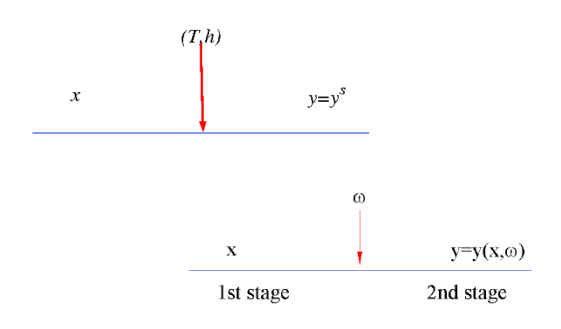
\includegraphics{hinh2.png}
        \caption{Cái nhìn cơ bản về quy hoạch ngẫu nhiên hai giai đoạn}
    \end{figure}
%%%%%%%%%%%%%%%%%%%%%%%%%%%%%%%%%


\section{Quy hoạch tuyến tính ngẫu nhiên hai giai đoạn (Two-Stage Stochastic linear programming (2-SLP))}
	\subsection{Mô hình QHTT ngẫu nhiên hai giai đoạn có phản hồi (Two-stage SLP Recourse model) - dạng đơn giản}
	\textbf{Định nghĩa 5} (QHTT ngẫu nhiên hai giai đoạn có phản hồi: 2-SLPWR).
    \textit{Quy hoạch tuyến tính ngẫu nhiên hai giai đoạn có phản hồi (2-SLPWR) hoặc chính xác hơn là có 
        phạt hành động khôi phục nói chung, được biểu diễn như sau}
    \begin{displaymath}
        2-SLP: \quad \underset{\boldsymbol{x \in \mathrm{X}}}{min} \; \boldsymbol{c}^T \cdot \boldsymbol{x} +
        \underset{\boldsymbol{y(\omega) \in \mathrm{Y}}}{min} \mathbf{E_{\omega}}[\boldsymbol{q \cdot y}]
    \end{displaymath}
    \textit{hoặc nói chung là}
    \begin{gather}
        2-SLP: \quad \underset{\boldsymbol{x \in \mathrm{X}, \: y(\omega) \in \mathrm{Y}}}{min}
        \mathbf{E_{\omega}}[\boldsymbol{c}^T \cdot \boldsymbol{x} + v(\boldsymbol{\mathrm{x, \omega}})]
    \end{gather}
    \textit{với} $v(\boldsymbol{\mathrm{x, \omega}}) \mathrel{:=} \boldsymbol{q \cdot y}$\\
    phụ thuộc vào
    \begin{gather*}
        A\boldsymbol{x}=\boldsymbol{b} \quad \quad \text{Các ràng buộc giai đoạn đầu,}\\
        T(\boldsymbol{\omega}) \cdot \boldsymbol{x} + W \cdot \boldsymbol{y(\omega)} = h(\boldsymbol{\omega}) \quad \text{Các ràng buộc giai đoạn hai}\\
        \text{hoặc gọn hơn là} \quad W \cdot \boldsymbol{y} = h(\boldsymbol{\omega}) - T(\boldsymbol{\omega}) \cdot \boldsymbol{x}
    \end{gather*}
    \begin{itemize}
        \item QHTT ngẫu nhiên này chỉ định 2-SP (ở công thức (2)) thành mục tiêu - một hàm 
        \textit{mục tiêu lớn ngẫu nhiên} cụ thể $g(\boldsymbol{x})$ có
        \begin{enumerate}
            \item hàm xác định $f(\boldsymbol{x})$ - tuyến tính, vẫn đang được tính toán
            \item một hàm xác suất $v(\boldsymbol{\mathrm{x}, \omega})$ \underline{có liên quan đến các kịch bản $\boldsymbol{\omega}$ khác nhau}.
        \end{enumerate}
        \item $\boldsymbol{y=y(x, \omega)} \in \mathbb{R}_+^p$ có tên là biến hành động phản hồi cho biến $\boldsymbol{x}$
            và là hiện thực hóa của $\boldsymbol{\omega}$
    \end{itemize}
    Hành động phản hồi này được xem như là phạt các hành động khôi phục trong QHTT ngẫu nhiên.\\
	Việc phạt khôi phục được biểu diễn thông qua giá trị trung bình $Q(\boldsymbol{\mathrm{x}})
    =\mathbf{E}_{\omega}[v(\boldsymbol{\mathrm{x}},\boldsymbol{\omega})]$\\
    \\
    \textbf{Cách tiếp cận 2: Phân tích kịch bản}\\
    \textbf{Giá trị kì vọng} $Q(\mathrm{x})$ rõ ràng là dành cho phân phối rời rạc $\boldsymbol{\omega}$\\
    Vì vậy, ta lấy $\Omega = \{ \omega_k \}$ là tập hữu hạn có kích thước S (có hữu hạn số lượng các kịch bản
        $\omega_1, \dots , \omega_S \in \Omega$, với khối lượng xác suất $p_k$ tương ứng).\\
    Bởi $\boldsymbol{y=y(x, \omega)}$ nên giá trị kì vọng của $v(\boldsymbol{y})=v(\boldsymbol{\mathrm{x, \omega}}) \mathrel{:=} \boldsymbol{q \cdot y}$
        (một $q$ cho tất cả $y_k$) là
    \begin{gather}
        Q(\boldsymbol{\mathrm{x}}) = \mathbf{E}_{\omega}[v(\boldsymbol{\mathrm{x}},\boldsymbol{\omega})] =
        \sum_{k=1}^{S} p_k \: q \: y_k = \sum_{k=1}^{S} p_k \: v(\boldsymbol{\mathrm{x}},\omega_k)
    \end{gather}
    trong đó\\
    \begin{itemize}
        \item $p_k$ là mật độ của kịch bản $\omega_k$, $q$ là phí phạt đơn vị đơn,\\
        \item và $q \: y_k = v(\boldsymbol{\mathrm{x}},\omega_k)$ - phí phạt của việc 
            sử dụng $y_k$ đơn vị trong pha phục hồi,\\
            phụ thuộc vào cả quyết định giai đoạn đầu $\boldsymbol{\mathrm{x}}$ và các kịch bản ngẫu nhiên $\omega_k$.
    \end{itemize}

	\subsection{Mô hình QHTT ngẫu nhiên hai giai đoạn có phản hồi (Two-stage SLP Recourse model) - dạng chính tắc}
	\textbf{Định nghĩa 6:} QHTT ngẫu nhiên hai giai đoạn có phản hồi (2-SLPWR) dạng chính tắc có thể biểu diễn như sau
    \begin{gather*}
        2-SLP: \quad \underset{x}{min} \: g(\boldsymbol{x}) \; \text{với}\\
        g(\boldsymbol{x}) \mathrel{:=} \boldsymbol{c}^T \cdot \boldsymbol{x} + v(\boldsymbol{y})\\
        \text{phụ thuộc vào} \quad A\boldsymbol{x}=\boldsymbol{b} \quad \text{trong đó} \quad \boldsymbol{x} \in \boldsymbol{\mathrm{X}} \subset \mathbb{R}^n, \; \boldsymbol{x \geq 0} \\
        v(\boldsymbol{z}) \mathrel(:=) \underset{\boldsymbol{y} \in \mathbb{R}_+^p}{min} \; \boldsymbol{q \: y} \quad \text{phụ thuộc vào} \quad
            W \cdot \boldsymbol{y} = h(\boldsymbol{\omega}) - T(\boldsymbol{\omega}) \cdot \boldsymbol{x} \mathrel{=:} \boldsymbol{z} 
    \end{gather*}
    trong đó $v(\boldsymbol{y}) \mathrel{:=} v(\boldsymbol{\mathrm{x}, \omega})$ là hàm giá trị giai đoạn hai, và\\
    $\boldsymbol{y}=\boldsymbol{y}(\boldsymbol{x}, \omega) \in \mathbb{R}_+^p$ là hành động phản hồi cho quyết
        định $\boldsymbol{x}$ và hiện thực hóa $\boldsymbol{\omega}$
    \begin{enumerate}
        \item Chi phí phản hồi kì vọng của quyết định x là $Q(\boldsymbol{\mathrm{x}}) \mathrel{:=} 
        \mathbf{E}_{\omega}[v(\boldsymbol{\mathrm{x}},\boldsymbol{\omega})]$ bằng phương trình (5). Vậy nói chung là,
        chúng ta tối thiểu hóa tổng chi phí kì vọng $min_{\boldsymbol{x} \in \mathbb{R}^n, \; \boldsymbol{y} \in \mathbb{R}_+^p}
            \; \boldsymbol{c}^T \cdot \boldsymbol{x} + Q(\boldsymbol{\mathrm{x}})$.
        \item Ta thiết kế các biến quyết định thứ hai $\boldsymbol{y(\omega)}$ vì thế chúng ta có thể điều chỉnh
            phản ứng với các ràng buộc ban đầu theo một cách thông minh!\\
            \begin{displaymath}
                \boldsymbol{\mathrm{x}}------T, h, \omega ------>\boldsymbol{y}
            \end{displaymath}
        \item Giá trị tối ưu của bài toán QHTT hai giai đoạn là
            $v_*=v(\boldsymbol{y}^*)$, \text{với} $\boldsymbol{y} = \boldsymbol{y}^*(\boldsymbol{x}, \omega)$ là nghiệm tối ưu,
            ở đây, $\boldsymbol{y}^* \in \mathbb{R}_+^p$. Giá trị tối ưu sau cùng là
            $\boldsymbol{c}^T \cdot \boldsymbol{x}^* + v(\boldsymbol{y}^*)$
    \end{enumerate}
    \textbf{BÀI TOÁN 1: [Công nghiệp - Sản xuất]}\\
    Xét một hãng công nghiệp \textbf{F} có một nhà máy sản xuất được n sản phẩm.\\
    Có nhiều bộ phận khác nhau (các bộ phận lắp ráp phụ) được đặt hàng từ \textit{m} bên thứ ba (the sites).
    Hình dưới đây cho thấy kế hoạch vận chuyển của hãng công nghiệp \textbf{F} với $m=3$ từ các nhà cung chấp
    và $n=4$ địa điểm sản xuất (the warehouses).
    \begin{figure}[ht]
        \centering
        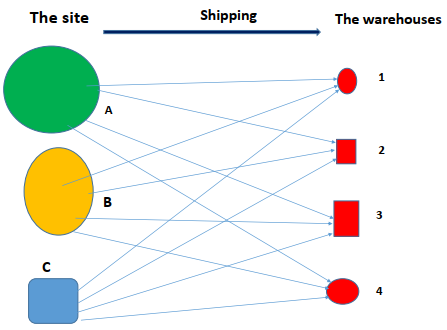
\includegraphics{hinh3.png}
    \end{figure}

    Một đơn vị sản phẩm $i$ cần $a_{ij} \geq 0$ bộ phận $j$, trong đó $i=1, \dots , n$ và $j = 1, \dots , m$.
    Nhu cầu về sản phẩm được mô hình hóa dưới dạng một vector ngẫu nhiên $\boldsymbol{\omega}=\boldsymbol{D}=(D_1,D_2, \dots , D_n)$.\\
    
    \textbf{Bài toán giai đoạn hai:}

    Với một giá trị khả kiến $\boldsymbol{d}=(d_1,d_2, \dots, d_n)$ của vector nhu cầu ngẫu nhiên $D$trên kia 
    , ta có thể tìm ra phương án sản xuất tốt nhất bằng cách giải bài toán QHTT ngẫu nhiên sau với
    \underline{các biến quyết định $\boldsymbol{z}=(z_1, z_2, \dots, z_n)$} - số lượng các đơn vị được sản xuất,

    và \underline{các biến quyết định \textbf{khác} $\boldsymbol{y}=(y_1, y_2, \dots, y_m)$} - số lượng các bộ phận còn trong kho.

    \begin{gather}
        LSP: \quad \underset{\boldsymbol{z, y}}{min} \; Z= \sum_{i=1}^{n} (l_i - q_i)z_i - \sum_{j=1}^{m}s_j y_j
    \end{gather}
    trong đó $s_j < b_j$ (được định nghĩa là giá đặt trước cho mỗi đơn vị bộ phận $j$), và

    $x_j, j=1, \dots, m$ là \underline{số lượng bộ phận được đặt trước khi sản xuất}.
    \begin{displaymath}
        \text{phụ thuộc vào}
        \begin{cases}
            y_j = x_j - \sum_{i=1}^{n}a_{ij}z_i, \quad j=1, \dots, m \\
            0 \leq z_i \leq d_i, \quad i=1, \dots, n; \quad y_j \geq 0, \; j=1, \dots, m
        \end{cases}
    \end{displaymath}

    Toàn bộ mô hình (của giai đoạn hai) có thể biểu diễn tương đương như sau
    \begin{gather}
        MODEL=
        \begin{cases}
            min_{\boldsymbol{z,y}} \: Z = \boldsymbol{c}^T \cdot \boldsymbol{z} - \boldsymbol{s}^T \cdot \boldsymbol{y}\\
            \text{với} \quad \boldsymbol{c} = (c_i \mathrel{:=} l_i - q_i) \quad \text{là hệ số chi phí}\\
            \boldsymbol{y}=\boldsymbol{x}-A^T \: \boldsymbol{z}, \text{trong đó} \; A=[a_{ij}] \; \text{là ma trận có kích thước $n \times m$}\\
            0 \leq \boldsymbol{z} \leq \boldsymbol{d}, \quad \boldsymbol{y} \geq 0
        \end{cases}
    \end{gather}
    
    Quan sát lời giải của bài toán, các vector $\boldsymbol{z, y}$ phụ thuộc vào hiện thực hóa $d$ của nhu cầu ngẫu nhiên
    $\boldsymbol{\omega = D}$ cũng như quyết định giai đoạn đầu $\boldsymbol{x}=(x_1,x_2, \dots , x_m)$.\\

    \textbf{Bài toán giai đoạn một:}

    Toàn bộ mô hình 2-SLPWR dựa trên một quy luật phổ biến là \textbf{sản xuất} $\geq$ \textbf{nhu cầu}.

    Bây giờ áp dụng cách tiếp cận dựa trên phân phối, cho $Q(\boldsymbol{x}) \mathrel{:=} \mathbf{E}[Z(\boldsymbol{z, y})]= \mathbf{E_{\boldsymbol{\omega}}}[\boldsymbol{x, \omega}]$
    biểu thị giá trị tối ưu của bài toán (6).
    
    \underline{$\boldsymbol{b}=(b_1,b_2, \dots, b_m)$ được xây dựng từ chi phí đặt trước $b_j$ trên mỗi bộ phận $j$} (trước khi biết nhu cầu).
    Các đại lượng $x_j$ được xác định từ bài toán tối ưu hóa sau
    \begin{gather}
        min \: g(\boldsymbol{\mathrm{x}, y, z}) = \boldsymbol{b}^T \cdot \boldsymbol{x} + Q(\boldsymbol{x}) =
        \boldsymbol{b}^T \cdot \boldsymbol{x} + \mathbf{E}[Z(\boldsymbol{z})]
    \end{gather}
    trong đó $Q(\boldsymbol{x})=\mathbf{E_\omega}[Z]=\sum_{i=1}^{n}p_i \: c_i \: z_i$ được lấy từ phân phối xác suất $\boldsymbol{\omega = D}$.

    Phần đầu của hàm mục tiêu biểu diễn \textbf{chi phí đặt trước} và $x$. Ngược lại, phần thứ hai biểu diễn \textbf{chi phí kì vọng}
    \underline{kế hoạch sản suất tối ưu} (7), được đưa ra bởi đại lượng đặt hàng thêm $z$, đã sử dụng nhu cầu ngẫu nhiên $\boldsymbol{D=d}$ cùng mật độ.

\section{Câu hỏi 1 BTL 2023}
    \subsection{Giới thiệu}
    \begin{itemize}
        \item Một bài toán quy hoạch tuyến tính ngẫu nhiên (Stochastic linear program) là một bài toán quy hoạch tuyến tính, trong đó:
            \begin{itemize}
                \item Hàm mục tiêu và các phương trình ràng buộc phải ở dạng tuyến tính.
                \item Phải có các tham số là yếu tố không chắc chắn và biết được xác suất của nó (biến ngẫu nhiên).
            \end{itemize}
        \item Cách giải bài toán quy hoạch tuyến tính ngẫu nhiên:
        
        Cho các tham số là các biến ngẫu nhiên rời rạc
            \begin{itemize}
                \item Bước 1: Xác định hàm mục tiêu
                \item Bước 2: Xác định các ràng buộc
                \item Bước 3: Xác định biến cố có thể xảy ra, ứng với mỗi biến cố, xác định giá trị các tham số ngẫu nhiên và xác suất xảy ra các biến cố đó.
                \item Bước 4:
                    \begin{itemize}
                        \item Cách 1: Ứng với từng biến cố, giải bài toán tối ưu bằng phương pháp đơn hình (simplex method). Tìm ra nghiệm tối ưu cho từng bài toán đó.
                        \item Cách 2: Tổng hợp các biến cố trong hàm mục tiêu để giải ra nghiệm tối ưu duy nhất cho tất cả các biên cố
                    \end{itemize}
                \item Bước 5: Kết luận giá trị cuối cùng của nghiệm tối ưu (giá trị kỳ vọng) của bài toán.
            \end{itemize}
    \end{itemize}

    \subsection{Cách giải}
    \textbf{Đề bài:} Xác định số lượng sản phẩm cần sản xuất đáp ứng nhu cầu thị trường sao cho lợi nhuận được tối ưu nhất\\
    \textbf{Giải:} Định nghĩa các thành phần trong bài toán như sau:
        \begin{itemize}
            \item $z \in \mathbb{R}^n$: số lượng sản phẩm từng loại (n loại sản phẩm)
            \item $x \in \mathbb{R}^m$: số lượng nguyên liệu có sẵn từng loại (m loại nguyên liệu)
            \item $A \in \mathbb{R}^{n*m}$: ma trận phụ thuộc giữa số sản phẩm cần sản xuất và số nguyên liệu cần sản xuất
                
            Trong đó, phần tử $a_{ij}$ là số nguyên liệu loại j cần để sản xuất một sản phẩm loại i $\rightarrow z=Ax$
            \item $c \in \mathbb{R}^m$: chi phí mua từng loại nguyên liệu
                \begin{itemize}
                    \item Chi phí mua một loại nguyên liệu M: $c_M = c_i x_i$
                    \item Chí phí mua tất cả nguyên liệu: $C_M = \sum c_i x_i = c^T x$
                \end{itemize}
            \item $l \in \mathbb{R}^n$: chi phí để sản xuất một sản phẩm từng loại
                \begin{itemize}
                    \item Chi phí sản xuất loại sản phẩm: $c_P = l_i z_i$
                    \item Chi phí sản xuất tất cả sản phẩm: $C_P = \sum l_i z_i = l^T z$
                \end{itemize}
            \item $q \in \mathbb{R}^n$: giá bán cho một sản phẩm từng loại
                \begin{itemize}
                    \item Doanh thu: $R = \sum q_i z_i = q^T z$
                    \item Lợi nhuận: $P = R - C_M - C_P = q^Tz - c^Tx - l^Tz = (q^T - l^T)z - c^Tx$
                \end{itemize}
            \item $y \in \mathbb{R}^m$: số lượng nguyên liệu còn lại $y = x - A^Tz$
            \item $s \in \mathbb{R}^m$: giá bán cho từng loại nguyên liệu thừa
                \begin{itemize}
                    \item Doanh thu từ việc bán nguyên liệu thừa: $R_M = \sum s_iy_i = s^Ty$
                \end{itemize}
            \item Lợi nhuận thực mà công ty thu được: $f(z) = (R - C_M - C_P) + R_M = (q^T = l^T)z - c^Tx + s^Ty$\\
                \begin{displaymath}
                    \text{phụ thuộc vào}
                    \begin{cases}
                        y = x - A^Tz\\
                        0 \leq z \leq d \text{(nhu cầu - demand)}\\
                        x \geq 0; \; y \geq 0
                    \end{cases}
                \end{displaymath}
        \end{itemize}

        \underline{Xét các kịch bản xảy ra:}
            
        $d^k \in \mathbb{R}^n$: nhu cầu thị trường trong kịch bản k

        $p^k$: xác suất xảy ra của biến cố k

        Trong một biến cố k cụ thể nào đó, ta có bài toán:
        \begin{displaymath}
            Max \; f(z^k) = (q^T - l^T)z^k - c^Tx + s^Ty^k\\
        \end{displaymath}
        \begin{displaymath}
            \text{phụ thuộc vào}
            \begin{cases}
                y^k = x - A^Tz^k\\
                0 \leq z^k \leq d^k\\
                x \geq 0; \; y^k \geq 0
            \end{cases}
        \end{displaymath}
        \hspace*{1cm} $\rightarrow$ Nghiệm tối ưu: $z = \sum p^k z^k$\\
        \hspace*{1cm} $\rightarrow$ Giá trị tối ưu: $f(z) = (q^T - l^T)z - c^Tx + s^Ty$\\

        \underline{Biến đổi bài toán thành dạng tổng hợp các kịch bản, ta được:}
        \begin{gather*}
            Max \; f(z^k) = \sum p^k((q^T - l^T)z^k - c^Tx + s^Ty^k)\\
            \Longleftrightarrow Max \; f(z^k) = \sum p^k((q^T - l^T)z^k + s^Ty^k) - c^Tx\\
            \text{phụ thuộc vào}
            \begin{cases}
                y^k = x - A^Tz^k\\
                0 \leq z^k \leq d^k\\
                x \geq 0; \; y^k \geq 0
            \end{cases}
        \end{gather*}

        \underline{Biến đổi bài toán về dạng chuẩn (standard form):}
        \begin{gather*}
            Min \; -f(z^k) = c^Tx - \sum p^k((q^T - l^T)z^k + s^Ty^k)\\
            \text{phụ thuộc vào}
            \begin{cases}
                y^k = x - A^Tz^k\\
                0 \leq z^k \leq d^k\\
                x \geq 0; \; y^k \geq 0
            \end{cases}
        \end{gather*}

        \subsection{Thành lập bài toán cụ thể theo như yêu cầu câu hỏi 1}

        Một công ty F sản xuất thực phẩm gồm 5 loại sản phẩm, 8 loại nguyên liệu được cho như bảng dưới đây, trong đó nhu cầu thị trường là ngẫu nhiên, nhưng theo đề bài nó là dạng phân phối nhị thức (kết cục chỉ xảy ra một trong hai biến cố) và xác suất cho mỗi biến cố là p = 0.5.
        \begin{figure}[!ht]
            \centering
            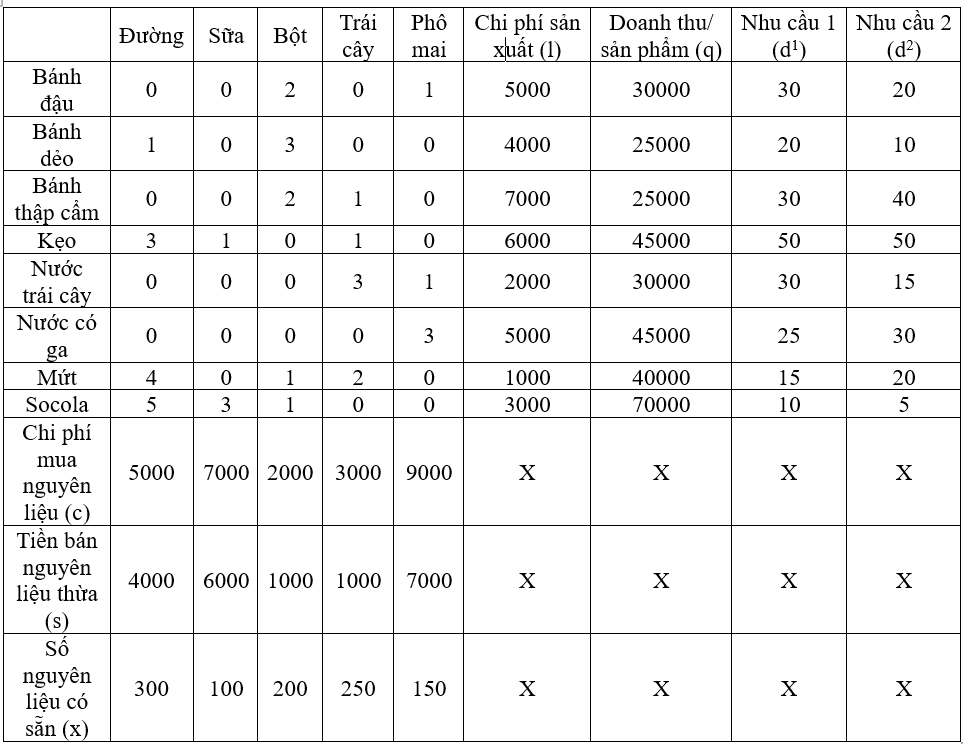
\includegraphics[width=1\linewidth]{tab1.png}
        \end{figure}

        Như các đinh nghĩa trong bài toán đã nêu ở phần II, ta có:
        \begin{gather*}
            x =
            \begin{pmatrix}
                300 & 100 & 200 & 250 & 150
            \end{pmatrix}\\
            A =
            \begin{pmatrix}
                0 & 0 & 2 & 0 & 1\\
                1&0&3&0&0\\
                0&0&2&1&0\\
                3&1&0&1&0\\
                0&0&0&3&1\\
                0&0&0&0&3\\
                4&0&1&2&0\\
                5&3&1&0&0\\
            \end{pmatrix}\\
            \text{c =}
            \begin{pmatrix}
                5000 & 7000 & 2000 & 3000 & 9000
            \end{pmatrix}\\
            l=
            \begin{pmatrix}
                5000\\
                4000\\
                7000\\
                6000\\
                2000\\
                5000\\
                1000\\
                3000\\
            \end{pmatrix}
            \quad \quad \quad q=
            \begin{pmatrix}
                30000\\
                25000\\
                25000\\
                45000\\
                30000\\
                45000\\
                40000\\
                70000\\
            \end{pmatrix}\\
            y=x-A^Tz
        \end{gather*}
        
        Model cụ thể của bài toán sẽ là:
        \begin{gather*}
            Min \; -f(z) = c^Tx - 0.5((q^T - l^T)z^1+s^Ty^1) - 0.5((q^T - l^T)z^2+s^Ty^2)\\
            \text{phụ thuộc vào}
            \begin{cases}
                y^1 = x - A^Tz^1\\
                y^2 = x - A^Tz^2\\
                0 \leq z^1 \leq d^1\\
                0 \leq z^2 \leq d^2\\
                x \geq 0; \; y^1 \geq 0; \; y^2 \geq 0
            \end{cases}
        \end{gather*}

        Giải bài toán bằng Excel, các số liệu được tổ chức theo bảng như sau:
        \begin{figure}[!ht]
            \centering
            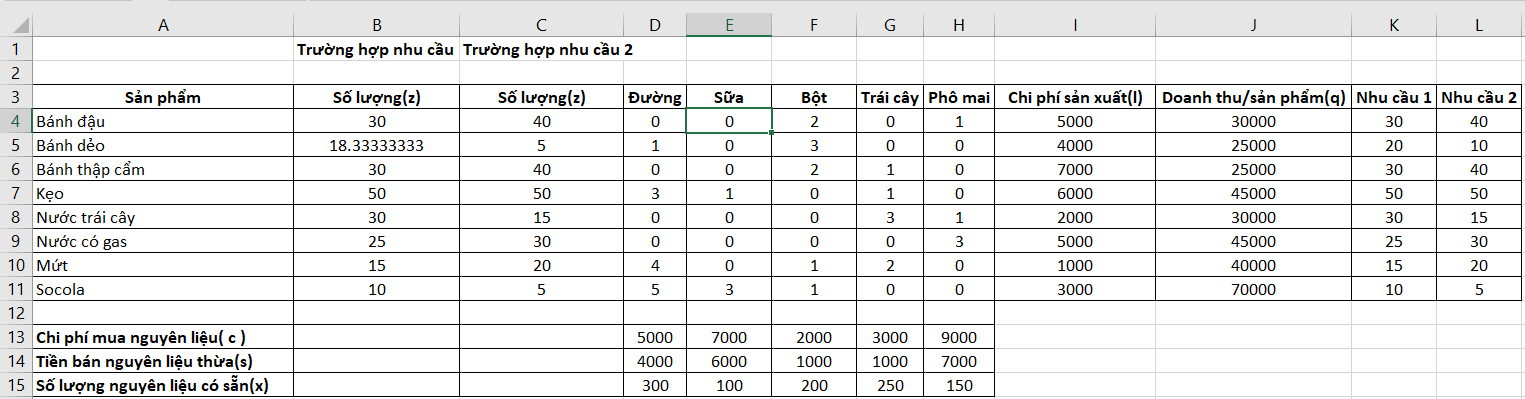
\includegraphics[width=1\linewidth]{tab2.png}
            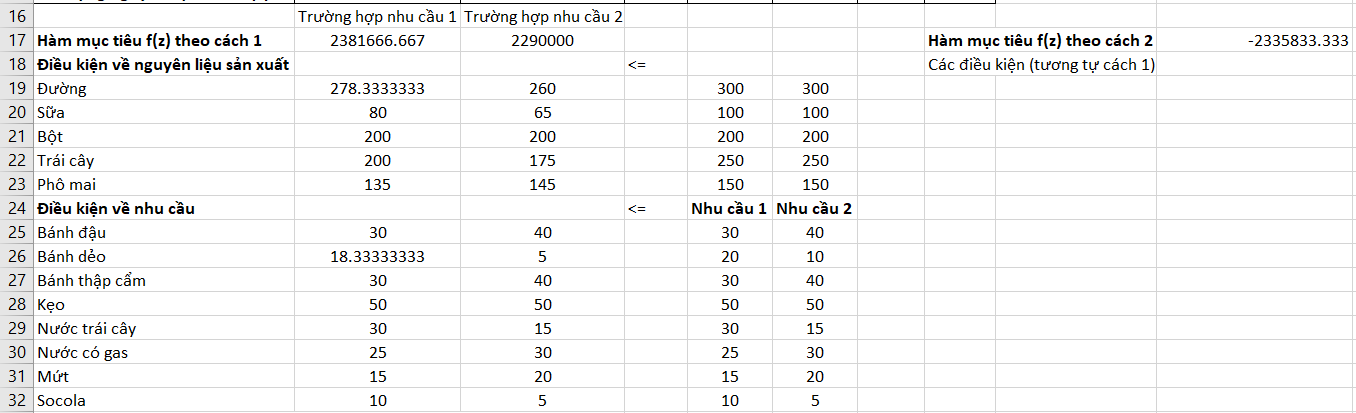
\includegraphics[width=1\linewidth]{tab3.png}
        \end{figure}

        Trong đó:
        \begin{itemize}
            \item Hàm mục tiêu ở ô B17 = SUMPRODUCT((J4:J11-I4:I11)*B4:B11)-\\
            SUMPRODUCT(D15:H15*D13:H13)+(D15-SUMPRODUCT(B4:B11*D4:D11))*D14+\\
            (E15-SUMPRODUCT(B4:B11*E4:E11))*E14+(F15-SUMPRODUCT(B4:B11*F4:F11))*F14+\\
            (G15-SUMPRODUCT(B4:B11*G4:G11))*G14+(H15-SUMPRODUCT(B4:B11*H4:H11))*H14
            \item Hàm mục tiêu ở ô C17 = SUMPRODUCT((J4:J11-I4:I11)*C4:C11)-\\
            SUMPRODUCT(D15:H15*D13:H13)+(D15-SUMPRODUCT(C4:C11*D4:D11))*D14+(E15-SUMPRODUCT(C4:C11*E4:E11))*E14+(F15-SUMPRODUCT(C4:C11*F4:F11))*F14+\\
            (G15-SUMPRODUCT(C4:C11*G4:G11))*G14+(H15-SUMPRODUCT(C4:C11*H4:H11))*H14
            \item Hàm mục tiêu ở ô J17 = SUMPRODUCT(D15:H15*D13:H13) - \\
            0.5*(SUMPRODUCT((J4:J11-I4:I11)*B4:B11) + (D15-SUMPRODUCT(B4:B11*D4:D11))*D14\\
            +(E15-SUMPRODUCT(B4:B11*E4:E11))*E14+(F15-SUMPRODUCT(B4:B11*F4:F11))*F14\\
            +(G15-SUMPRODUCT(B4:B11*G4:G11))*G14+(H15-SUMPRODUCT(B4:B11*H4:H11))*H14) - 0.5*(SUMPRODUCT((J4:J11-I4:I11)*C4:C11) + (D15-SUMPRODUCT(C4:C11*D4:D11))*D14\\
            +(E15-SUMPRODUCT(C4:C11*E4:E11))*E14+(F15-SUMPRODUCT(C4:C11*F4:F11))*F14\\
            +(G15-SUMPRODUCT(C4:C11*G4:G11))*G14+(H15-SUMPRODUCT(C4:C11*H4:H11))*H14)
        \end{itemize}

        Sử dụng chức năng Solver ở mục Data ta giải được bài toán với kết luận như sau:
        \begin{figure}[!ht]
            \centering
            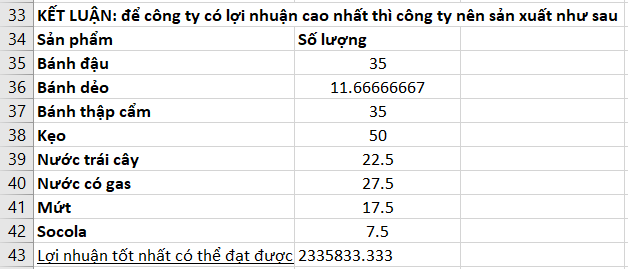
\includegraphics[width=1\linewidth]{tab4.png}
        \end{figure}

        Nhận xét: khi giải bài toán bằng 2 cách như đã nêu ở phần II, ta thu được kết quả giống nhau.

\section{Câu hỏi 2 BTL 2023}
    \subsection{Đề bài}
    Tìm hiểu, triển khai và xác minh tính hiệu quả của thuật toán đã nghiên cứu hoặc giải quyết mô hình lập kế hoạch sơ tán ngẫu nhiên hai giai đoạn trên mạng lưới nhỏ, với cách tiếp cận thiết kế thí nghiệm. Mô phỏng sẽ có tối đa 50 nút và 100 liên kết.
    
    \subsection{Giới thiệu}
    
    Các sự kiện cực đoan (do thiên tai hoặc do con người gây ra) như động đất, lũ lụt, lốc xoáy,… có thể ảnh hưởng nghiêm trọng đến mạng lưới và dịch vụ viễn thông ở các khu vực đô thị. 
    Lập kế hoạch sơ tán hợp lý sao cho những thảm họa là một hành động quan trọng và cần được suy nghĩ cẩn thận (sớm) và thực hiện (vào ngày nào, thời gian nào), đặc biệt khi có sự không chắc chắn. 
    
    Bài tập lớn này sẽ nghiên cứu rõ hơn bài báo của L. Wang, “A two-stage stochastic programming framework for evacuation planning in disaster responses,”(2020) về giải pháp kế hoạch sơ tán cụ thể cho những người bị ảnh hưởng từ khu vực nguy hiểm sang khu vực an toàn.
    Vì có rất nhiều tình huống cũng như những thiệt hại phát sinh trong thảm họa do đó vấn đề sơ tán này nên được coi là một vấn đề quy hoạch ngẫu nhiên.
    Quy hoạch ngẫu nhiên có phản hồi được sử dụng để tìm ra các quyết định không dự đoán được phải được thực hiện trước khi biết được các thực hiện của một số biến ngẫu nhiên sao cho tổng chi phí kỳ vọng của các hành động hậu quả có thể là nhỏ nhất.
    Dựa trên phân tích trên, vấn đề sơ tán trong bài tập lớn này được xây dựng thành một mô hình quy hoạch ngẫu nhiên hai giai đoạn dựa trên kịch bản để đại diện cho sự ngẫu nhiên xuất phát từ cường độ và ảnh hưởng.

    \subsection{Mục tiêu}

    Lập kế hoạch sơ tán người dân khỏi những khu vực bị ảnh hưởng bởi các thiên tai như lũ lụt, động đất, núi lửa,...
    Mô hình quy hoạch ngẫu nhiên hai giai đoạn xem xét cả lựa chọn trước đường sơ tán (trước thảm họa) và thích ứng (sau thảm họa) để cung cấp kế hoạch sơ tán trước mắt cho người bị ảnh hưởng từ các khu vực nguy hiểm sang các khu vực an toàn.
    Không giống như các mô hình xác định, nó liên quan đến sự khả dụng của các thời gian di chuyển và khả năng liên kết ngẫu nhiên dựa trên kịch bản.
    Trong giai đoạn thứ nhất, giả sử rằng người bị ảnh hưởng không thể thu thập được thông tin về mức độ thiên tai và mức độ hư hại của đường và sau một khoảng thời gian nhất định, họ có thể thu thập được thông tin mạng lưới đường bộ chính xác thông qua một số thiết bị giám sát thời gian thực sau đó thực hiện kế hoạch sơ tán nhanh cho tất cả các mức độ thảm họa.
    Các quyết định giai đoạn thứ hai (hậu quả) được phụ thuộc vào các quyết định giai đoạn đầu, được thực hiện sau khi thực hiện các thời gian di chuyển và khả năng ngẫu nhiên.
    Do đó, mục tiêu là thực hiện kế hoạch sơ tán trước khi tối ưu hóa trong giai đoạn đầu, dưới các điều kiện không chắc chắn sẽ phải đối mặt trong giai đoạn thứ hai.
    Hơn nữa, thay vì quyết định vị trí cơ sở và đặt trước hàng hóa cứu trợ khẩn cấp, kế hoạch này trình bày đường sơ tán cụ thể cho người bị ảnh hưởng. 

    \subsection{Các bước thực hiện}

    \begin{itemize}
        \item Bước 1: Đề xuất mô hình lập trình ngẫu nhiên hai giai đoạn và lựa chọn lộ trình trước và sau thảm họa để cung cấp kế hoạch sơ tán cho những người bị ảnh hưởng đến nơi an toàn.
        \item Bước 2: Xây dựng kế hoạch di chuyển rõ ràng của những người dân bị ảnh hưởng bằng mô hình dòng chi phí tối thiểu từ đó chia thành 2 bài toán nhỏ là luồng có chi phí nhỏ nhất và bài toán phụ thuộc vào thời gian của nó.
        \item Bước 3: Để thu được nghiệm gần tối ưu, khung thuật toán tối ưu hóa đạo hàm riêng được sử dụng để giảm dần khoảng cách tương đối của giới hạn trên và dưới, tức là các giá trị mục tiêu của mô hình gốc và mô hình độc lập; và hai bài toán con được giải quyết bằng thuật toán đường liên tục ngắn nhất. 
    \end{itemize}

    \subsection{Bảng kí hiệu}

    \begin{center}
        \begin{tabular}{ll}
            \toprule
            Kí hiệu & Ý nghĩa\\
            \midrule
            V & tập hợp các nút (nodes)\\
            A & tập hợp các liên kết (links)\\
            i, j & vị trí của các nút, i, j $\in$ V\\
            (i,j) & vị trí của các liên kết, (i,j) $\in$ A\\
            s & số thứ tự của kịch bản\\
            S & tổng số kịch bản\\
            v & giá trị cung cấp của nút nguồn\\
            T & tổng số khoảng thời gian\\
            $u_{ij}$ & dung lượng trên liên kết (i,j)\\
            $u\dfrac{s}{ij}(t)$ & dung lượng trên liên kết (i,j) trong kịch bản s ở thời gian t\\
            $c\dfrac{s}{ij}(t)$ & thời gian di chuyển trên liên kết (i,j) trong kịch bản s ở thời gian t\\
            $\mu_s$ & xác suất trong kịch bản s\\
            \bottomrule
        \end{tabular}
        
        \begin{tabular}{ll}
            \toprule
            Biến quyết định & Ý nghĩa\\
            \midrule
            $x_{ij}$ & luồng trên liên kết (i,j)\\
            $y\dfrac{s}{ij}$ & luồng trên liên kết (i,j) trong kịch bản s ở thời gian t\\
            \bottomrule
        \end{tabular}
    \end{center}

    \subsection{Các ràng buộc}

    \textbf{Giai đoạn 1:}

    Trong giai đoạn đầu tiên, một sơ tán khả thi cần được xác định từ vùng nguy hiểm đến vùng an toàn. Mỗi luồng trên mỗi liên kết cần thỏa mãn ràng buộc về cân bằng luồng (tổng luồng chạy vào một nút bằng tổng luồng chạy ra khỏi nút đó)
    \begin{gather*}
        \sum\limits_{(i,j) \in A} x_{ij} - \sum\limits_{(j,i) \in A} x_{j,i} = d_i\\
        \text{trong đó $d_i$ là tham số, với $d_i =$}
        \begin{cases}
            v,i = s \\
            -v,i = t\\
            0, \text{các trường hợp còn lại}
        \end{cases}
    \end{gather*}

    Ngoài ra luồng còn phải thỏa mãn ràng buộc về dung lượng tối đa (luồng trên mỗi liên kết không vượt quá dung lượng tối đa của liên kết đó)
    \begin{displaymath}
        0 \leq x_{ij} \leq u_{ij}, \forall (i,j) \in A
    \end{displaymath}

    Lưu ý:  Phạt liên kết (link penalty) $p_{ij}$ $\in A$ là một giá trị được gán cho mỗi liên kết để đánh giá mức độ không mong muốn của việc sử dụng liên kết đó trong một cách sơ tán. Hàm liên kết có thể định nghĩa là
    \begin{displaymath}
        f(\boldsymbol{\mathrm{X}}) = \sum\limits_{(i,j) \in A} p_{ij}x_{ij}
    \end{displaymath}
    \begin{gather*}
        \text{trong đó} \;
        \boldsymbol{\mathrm{X}} \mathrel{:=} (x_{ij})_{(i,j) \in A}
    \end{gather*}

    \textbf{Giai đoạn 2:}

    Ở giai đoạn 2, những người bị ảnh hưởng sẽ nhận được các đường đi ứng với thời gian sơ tán tối thiểu theo thông tin thảm họa thời gian thực. 
    Trước thời điểm đó, những người bị ảnh hưởng sẽ được sơ tán theo kế hoạch sơ tán giai đoạn một quy định lúc trước; nói cách khác, kế hoạch sơ tán ở các kịch bản khác nhau trước thời điểm đều giống như tiên nghiệm. 
    Theo thảo luận ở trên, các ràng buộc cho kế hoạch sơ tán của từng kịch bản trước ngưỡng thời gian có thể được xây dựng như sau:
    \begin{displaymath}
        y_{ij}^s(t) = x_{ij}, \quad \forall t \leq \Tilde{T}, (i,j) \in A, s = 1, 2, \dots, S
    \end{displaymath}

    Các cặp ràng buộc thể hiện mối quan hệ giữa liên kết vật lí và cung không gian - thời gian trong kế hoạch sơ tán, 
    nghĩa là nếu có các luồng truy cập trên liên kết $(i,j)$ ví dụ $x_{ij}=2$ thì luồng truy cập trên mỗi liên kết trước thời điểm 2, $y\dfrac{s}{ij}(t)=2$. 
    Nói cách khác, trước ngưỡng đó, kế hoạch sơ tán trong mỗi kịch bản của giai đoạn thứ hai giống như kế hoạch sơ tán ban đầu ở giai đoạn đầu tiên. 
    Sau đây, một mô hình giai đoạn hai được thiết lập với mục tiêu nhằm giảm thiểu tổng thời gian di tản của những người bị ảnh hưởng khỏi khu vực nguy hiểm ở mỗi kịch bản: 

    \begin{gather}
        Q(Y,s) = min \sum\limits_{(i,j) \in A_s} c_{ij}^s \cdot y_{ij}^s(t)
    \end{gather}

    \hspace*{2.5cm} \text{Tùy thuộc vào}

    \begin{gather}
        \sum\limits_{(i_t,j_{t'}) \in A_s} y_{ij}^s(t) - \sum\limits_{(j_{t'},i_t) \in A_s} y_{ij}^s(t') = d_i^s(t), \forall i \in V, t \in \{0,1, \dotsc, T \}, s = 1, 2, \dots, S\\
        0 \leq y_{ij}^s(t) \leq u_{ij}^s(t), \forall (i,j) \in A_s, t \in \{0,1, \dotsc, T \}, s = 1, 2, \dots, S\\
        \sum\limits_{t \leq \Tilde{T}} y_{ij}^s(t) = x_{ij}, (i,j) \in A, s = 1, 2, \dots, S
    \end{gather}

    \begin{itemize}
        \item Hàm mục tiêu (9) là thời gian sơ tán tổng thể của các phương tiện giao thông trong kịch bản giảm thiểu s
        \item Ràng buộc (10) là ràng buộc cân bằng luồng
        \item Ràng buộc (11) là ràng buộc về dung lượng tối đa 
        \item Ràng buộc (12) là một ràng buộc cặp để đảm bảo rằng kế hoạch sơ tán trong từng kịch bản ở giai đoạn thứ hai trước ngưỡng thời gian giống như kế hoạch tiên nghiệm ở giai đoạn đầu.
    \end{itemize}

    \subsection{Mô hình lập kế hoạch sơ tán ngẫu nhiên hai giai đoạn}

    Cần có được một kế hoạch sơ tán vững chắc trong giai đoạn đầu tiên bằng cách đánh giá các kế hoạch thích ứng ở giai đoạn thứ hai.
    Để đạt được mục tiêu này, kế hoạch sơ tán giai đoạn một với thời gian sơ tán tổng thể dự kiến của đường sơ tán ứng với từng kịch bản và xác suất xảy ra của từng kịch bản s giả định là $\mu_s, s = 1,2, \dotsc, S.$
    Để giảm thiểu mức phạt đối với kế hoạch sơ tán trước đó và tổng thời gian sơ tán dự kiến của mỗi kế hoạch sơ tán ứng theo kịch bản, mô hình kế hoạch sơ tán hai giai đoạn trong môi trường phụ thuộc thời gian và ngẫu nhiên được xây dựng như sau:
    
    \begin{displaymath}
        \begin{cases}
            min \; \sum\limits_{(i,j) \in A} p_{ij}x_{ij} + \sum_{s=1}^{S} \mu_s \cdot Q(Y,s)\\
            s.t.\\
            \sum\limits_{(i,j) \in A} x_{ij} - \sum\limits_{(j,i) \in A} x_{ji} = d_i, \forall i \in V\\
            0 \leq x_{ij} \leq u_{ij}, \forall (i,j) \in A\\
            \text{trong đó}\\
            Q(Y,s) = min \sum\limits_{(i,j) \in A_s} c_{ij}^s(t) \cdot y_{ij}^s(t)\\
            s.t.\\
            \sum\limits_{(i_t,j_{t'}) \in A_s} y_{ij}^s(t) - \sum\limits_{(j_{t'},i_t) \in A_s} y_{ij}^s(t') = d_i^s(t), \forall i \in V,\\
            t \in \{0,1, \dotsc, T \}, s = 1, 2, \dots, S\\
            0 \leq y_{ij}^s(t) \leq u_{ij}^s(t), \forall (i,j) \in A, t \in \{0,1, \dotsc, T \}, s = 1, 2, \dots, S\\
            \sum\limits_{t \leq \Tilde{T}} y_{ij}^s(t) = x_{ij}, (i,j) \in A, s = 1, 2, \dots, S\\
        \end{cases} 
    \end{displaymath}

    \begin{gather}
        \begin{cases}
            min \; \sum\limits_{(i,j) \in A} p_{ij}x_{ij} + \sum_{s=1}^{S} (\mu_s \cdot \sum\limits_{(i,j) \in A_s} c_{ij}^s(t) \cdot y_{ij}^s(t))\\
            s.t.\\
            \sum\limits_{(i,j) \in A} x_{ij} - \sum\limits_{(j,i) \in A} x_{ji} = d_i, \forall i \in V\\
            0 \leq x_{ij} \leq u_{ij}, \forall (i,j) \in A\\
            \sum\limits_{(i_t,j_{t'}) \in A_s} y_{ij}^s(t) - \sum\limits_{(j_{t'},i_t) \in A_s} y_{ij}^s(t') = d_i^s(t), \forall i \in V,\\
            t \in \{0,1, \dotsc, T \}, s = 1, 2, \dots, S\\
            0 \leq y_{ij}^s(t) \leq u_{ij}^s(t), \forall (i,j) \in A, t \in \{0,1, \dotsc, T \}, s = 1, 2, \dots, S\\
            \sum\limits_{t \leq \Tilde{T}} y_{ij}^s(t) = x_{ij}, (i,j) \in A, s = 1, 2, \dots, S\\
        \end{cases}
    \end{gather}

    Để giải quyết mô hình (13) cần một mô hình lập trình nguyên vốn chứa hai loại biến quyết định là 
    $X \mathrel{:=} \{x_{ij}\} (i,j \in A)$ và $Y \mathrel{:=} \{y\dfrac{s}{ij}(t)\}(i,j \in A, s \in \{1,2, \dotsc, S\}, t \in \{1,2, \dotsc, T\})$
    Ta cần chia mô hình thành 2 bài toán nhỏ bằng phương pháp song phương nhằm nới lỏng ràng buộc ghép vào hàm mục tiêu bằng cách sử dụng phương pháp nới lỏng Lagrange. 
    Cụ thể, mô hình ban đầu được phân tách thành một bài toán luồng có chi phí nhỏ nhất và một bài toán phụ thuộc vào thời gian, 
    mà có thể được giải quyết hiệu quả bằng các thuật toán chính xác. Vấn đề then chốt của phương pháp nới lỏng Lagrange là tìm ra cận trên của bài toán cần quan tâm. 
    Các giải pháp nới lỏng, ngẫu nhiên, là khả thi cho bài toán ban đầu. 

    \subsection{Bài toán 1}

    \begin{displaymath}
        \begin{cases}
            min \; SP1(\alpha) = \sum\limits_{(i,j) \in A} (p_{ij} - \sum_{s=1}^{S}\sum\limits_{t \leq \Tilde{T}} \alpha_{ij}^s(t))x_{ij}\\
            s.t.\\
            \sum\limits_{(i,j) \in A} x_{ij} - \sum\limits_{(j,i) \in A} x_{ij} = d_i, \forall i \in V\\
            0 \leq x_{ij} \leq u_{ij}, \forall (i,j) \in A\\
        \end{cases}
    \end{displaymath}

    Cho một mạng G bao gồm n đỉnh và m cạnh mỗi cạnh có dung lượng A(e), chi phí trên mỗi luồng dọc theo cạnh là C(e) (số nguyên) và cân bằng đỉnh. 
    Tổng chi phí của bất kì luồng f có thể định nghĩa là:
    \begin{displaymath}
        A(f) = \sum\limits_{e \in E} A(e)f(e)
    \end{displaymath}

    Đối với một giá trị nhất định $K$, chúng ta phải tìm một luồng có đại lượng này và trong số tất cả các luồng có đại lượng này, chúng ta phải chọn luồng có chi phí thấp nhất. 
    Nhiệm vụ này được gọi là bài toán luồng chi phí tối thiểu.

    Nhiệm vụ này có thể giải quyết bằng thuật toán đường đi ngắn nhất liên tiếp.

    Đường đi ngắn nhất liên tiếp được xây dựng trên mạng luồng chung $G = (V,E)$ với dung lượng
    $f(.)$, giới hạn dưới, chi phí C(.) trên các cạnh và cân bằng (dòng vào bằng dòng ra tại bất kỳ nút nào). 
    Giả sử các điều dưới đây được thỏa mãn
    \begin{enumerate}
        \item Các cạnh có dung lượng không âm và giới hạn dưới bằng 0:
            \begin{displaymath}
                0 \leq f(u,v) \leq c(u,v) \quad \forall (u,v)
            \end{displaymath}
        \item Mọi luồng f phải thoả mãn ràng buộc bảo toàn số luồng vào bằng số luồng ra tại mỗi nút: 
            \begin{displaymath}
                \sum\limits_{v \in V} f(v,u) = \sum\limits_{v \in V} f(u,v) \leftrightarrow \sum\limits_{v \in V} f(v,u) - \sum\limits_{v \in V} f(u,v) = 0, \quad u \neq s,t
            \end{displaymath}
    \end{enumerate}

    \subsubsection{Thuật toán đường đi ngắn nhất liên tiếp}

    Mục tiêu của bài toán này là sẽ tìm kiếm giá trị lớn nhất của luồng và đồng thời tối ưu hóa hàm mục tiêu cho trước.
    \begin{itemize}
        \item Bước 1: Chọn biến x làm một luồng khả thi, tức là một luồng thỏa mãn các ràng buộc về dung lượng, đối xứng, và bảo toàn luồng. 
            Luồng này cũng phải có chi phí nhỏ nhất trong các luồng khả thi có cùng giá trị luồng.
        \item Bước 2: Kiểm tra xem luồng đã đạt giá trị mong muốn hay chưa, hoặc có còn đường đi nào có chi phí nhỏ hơn trong mạng lưới dư hay không.
            Mạng lưới dư là một mạng lưới được tạo ra bằng cách thêm các cung ngược lại vào mạng lưới ban đầu, với chi phí và dung lượng phù hợp.
            Nếu luồng đã đạt giá trị mong muốn v, hoặc không còn đường đi nào có chi phí nhỏ hơn, thuật toán kết thúc.
            Nếu không, tìm đường đi ngắn nhất với luồng lớn nhất trong mạng lưới dư, bằng cách sử dụng thuật toán nhãn sửa, và sau đó chuyển sang Bước 3.
            Hàm $A(x), C(x), U(x)$ trong phần còn lại mạng có thể được định nghĩa là:
            \begin{displaymath}
                A(x) = \{ (i,j) | (i,j) \in A, x_{ij} < u_{ij} \} \cup \{(j,i) | (j,i) \in A, x_{ij} > 0 \}\\
            \end{displaymath}
            \begin{displaymath}
                C(x)  = \begin{cases}
                    c_{ij}, (i,j) \in A, x_{ij} < u_{ij}\\
                    -c_{ji}, (j,i) \in A, x_{ji} > 0\\
                \end{cases}
            \end{displaymath}
            \begin{displaymath}
                U(x)  = \begin{cases}
                    u_{ij}, (i,j) \in A, x_{ij} < u_{ij}\\
                    x_{ji}, (j,i) \in A, x_{ji} > 0\\
                \end{cases}
            \end{displaymath}
        \item Bước 3: Tăng luồng dọc theo đường đi có chi phí nhỏ nhất, bằng cách thêm hoặc bớt luồng trên các cung thuộc đường đi đó. 
        Nếu giá trị luồng tăng không vượt quá giá trị mong muốn, quay lại Bước 2.
    \end{itemize}

    Lưu ý rằng trong vòng lặp cuối cùng của thuật toán, chỉ cần tăng luồng thêm một lượng sao cho giá trị luồng cuối không vượt quá K.

    \subsubsection{Thuật toán nhãn sửa (label correcting algorithm)}

    Đầu vào: Cho $G=(V,E)$ là một đồ thị (có thể vô hướng hoặc có hướng) và
    $\{ a_{ij}:(i,j) \in E \}$ là tập hợp các trọng số không âm trên các cạnh.
    Chúng ta phân biệt hai nút trong đồ thị, cụ thể là điểm gốc
    $s \in V$ và điểm đích $t \in V$. Nút
    $j \in V$ được gọi là nút con của nút $i \in V$ nếu có cạnh từ $i$ đến $j$.
    Lưu ý rằng nếu đồ thị vô hướng và $(i,j)$ là một cạnh, thì $i$ là con của $j$ và $j$ là con của $i$.
    Mục tiêu của chúng ta là tìm đường đi ngắn nhất từ $s$ đến $t$.
    
    Ý tưởng đằng sau các thuật toán sửa nhãn là tìm dần dần các đường đi ngắn hơn từ nguồn gốc của mọi nút khác i. 
    Điều này đạt được bằng cách duy trì nhãn di cho mỗi nút i, nhãn này biểu thị giới hạn trên của khoảng cách ngắn nhất từ điểm gốc s đến nút i. 
    Nhãn $d_t$ của đích t được duy trì trong một biến gọi là Upper. 
    Như chúng ta sẽ thấy, biến Upper đóng vai trò một vai trò đặc biệt trong thuật toán. 
    Khi thuật toán tiến triển, nếu một đường đi từ điểm gốc đến nút i được phát hiện và khoảng cách của nó nhỏ hơn di, thì nhãn của nút i sẽ được sửa. 
    Để tạo thuận lợi cho việc ghi sổ, thuật toán duy trì một danh sách các nút được gọi là Open. Danh sách Open chứa các nút sẽ được kiểm tra bởi
    thuật toán và là ứng cử viên có thể được đưa vào con đường ngắn nhất. Khi danh sách mở trống, thuật toán kết thúc.
    \begin{itemize}
        \item Bước 1: Cho $d_s = 0$, $d_i = \infty$ với $\forall i \in V \ \{s,t\}$ và $Upper = \infty$.
            Tạo danh sách $Open = \{s\}$
        \item Bước 2: Xóa a node i khỏi Open
        \item Bước 3: Với mỗi con j của i ta thực hiện:
            \begin{itemize}
                \item Nếu $d_i + a_{ij} < min (d_j, Upper), d_j = d_i + a_{ij}$ và cho i thành nút cha của j
                \item Nếu j khác đích t, thêm j vào danh sách Open nếu j chưa xuất hiện. Ngược lại nếu j là đích t, $Upper = d_i + a_{it}$
            \end{itemize}
        \item Bước 4: Nếu danh sách Open rỗng kết thúc thuật toán nếu không quay lại bước 2.
    \end{itemize}

    Về mặt hình thức, thuật toán sửa nhãn nói chung được đưa như trên.
    Ở bước 3 của thuật toán, chúng ta gặp một đường đi từ s đến j qua i và chúng ta kiểm tra xem đường dẫn này (i) có ngắn hơn đường đi được xem xét trước đây từ s đến j (tức là nếu 
    $d_i + a_{ij} < d_j$) và (ii) có khả năng dẫn đến a
    đường đi ngắn nhất từ s đến t (tức là nếu $d_i + a_{ij} < Upper$) hay không. 
    Nếu vậy thì nhãn dj bị giảm và nút j được đặt vào danh sách Open sao cho các đường đi qua j và tới các phần tử con của j có thể được kiểm tra sau.
    \begin{enumerate}
        \item Trong suốt thuật toán, nhãn $d_i$ của nút i tùy ý là $\infty$ (tương ứng
        trong trường hợp tôi chưa vào danh sách Open) hoặc đó là độ dài của một số đường dẫn từ s đến i bao gồm các nút đã vào danh sách Open ít nhất một lần.
        \item Nếu $d_i < \infty$, thì có thể thu được đường đi từ s đến i có độ dài di bằng cách truy tìm các nút cha bắt đầu với cha mẹ của i.
        \item Thuật toán sẽ kết thúc sau một số bước hữu hạn. Hơn nữa, khi nó kết thúc,
        biến Upper sẽ bằng khoảng cách ngắn nhất từ điểm gốc đến đích t (trường hợp này có ít nhất một đường đi từ s tới t), hoặc bằng 
        $\infty$ (trường hợp không có đường đi từ s đến t). 
        \item Nút j mà $d_i + a_{ij} \geq Upper$ ở bước 3 chắc chắn sẽ không được được đưa vào danh sách Open trong lần lặp hiện tại và có thể không được đưa vào danh sách trong bất kỳ lần lặp tiếp theo nào. 
        Do đó, số lượng nút vào danh sách Open có thể nhỏ hơn đáng kể so với tổng số nút. Đặc biệt, thuật toán sửa nhãn có thể được hiệu quả hơn thuật toán DP cơ bản.
    \end{enumerate}

    Lưu ý rằng ở bước 2 của Thuật toán 1, có một số quyền tự do trong việc chọn nút nào để loại bỏ từ danh sách Open trong mỗi lần lặp. Mỗi lựa chọn tương ứng với một cách triển khai khác nhau của thuật toán sửa nhãn. 
    Một số lựa chọn nổi tiếng hơn được đưa ra như sau:
    \begin{enumerate}
        \item Thuật toán BFS: Danh sách Open được duy trì dưới dạng hàng đợi FIFO,
            tức là nút luôn được xóa khỏi đầu Open và mỗi nút vào Open được đặt tại phần dưới cùng của Open.
        \item Thuật toán DFS: Danh sách Open được duy trì dưới dạng hàng đợi LIFO,
            tức là nút luôn được xóa khỏi đầu Open và mỗi nút vào Open được đặt tại đỉnh của Open.
        \item Thuật toán Tìm kiếm tốt nhất - Đầu tiên: Trong mỗi lần lặp, một nút có nhãn nhỏ nhất sẽ bị xóa khỏi danh sách. Đây được gọi là phương pháp Dijkstra. Có thể chỉ ra rằng trong phương pháp này,mỗi nút sẽ chỉ vào Open tối đa một lần
    \end{enumerate}

    \subsubsection{Giải thuật cho đồ thị vô hướng, đa đồ thị}

    Trong trường hợp đồ thị vô hướng hay đa đồ thị không khác nhau nhiều về mặt khái niệm của thuật toán trên. 
    Tuy nhiên, việc thực hiện thuật toán sẽ khó khăn hơn một chút.
    \begin{itemize}
        \item Đầu tiên, luồng cho từng cạnh phải giữ riêng biệt.
        \item Thứ hai, khi tìm kiếm đường đi ngắn nhất, cần phải tính đến việc điều quan trọng là cạnh nào trong số nhiều cạnh được sử dụng trong đường dẫn. 
            Do đó, thay vì mảng tổ tiên thông thường, chúng ta phải lưu trữ số cạnh mà chúng ta xuất phát cùng với mảng tổ tiên.
        \item Thứ ba, khi luồng tăng dọc theo một cạnh nhất định thì cần phải giảm luồng dọc theo cạnh sau. Vì chúng ta có nhiều cạnh nên chúng ta phải lưu trữ số cạnh của cạnh đảo ngược cho mỗi cạnh.
    \end{itemize}

    \subsubsection{Kết quả}

    \textbf{Đánh giá:}

    Thuật toán Dijkstra yêu cầu ít lần lặp hơn Bellman-Ford.Tuy nhiên, Bellman-Ford yêu cầu ít công việc hơn cho mỗi lần lặp.
    Ta có thể dừng thuật toán của Dijkstra sau khi đã xác định xong đến nút đích.
    Ta không thể sử dụng thuật toán của Dijkstra nếu có chi phí liên kết âm.
    Còn Bellman-Ford vẫn hoạt động.

    \textbf{Độ phức tạp:} phụ thuộc vào cấp số nhân của đầu vào, trong trường hợp xấu nhất nó có thể đẩy tối đa 1 đơn vị lưu lượng trên 1 lần lặp, 
    lấy O(F) lặp đi lặp lại để tìm ra luồng kích thước có chi phí tối thiểu F, 
    làm cho tổng thời gian chạy là O(F.T). T là thời gian cần để tìm đường đi ngắn nhất từ nguồn tới đích.

    Nếu thuật toán Bellman-Ford được sử dụng cho việc này, nó sẽ làm cho thời gian chạy là O(mn). 
    Cũng có thể sửa đổi thuật toán Dijkstra để nó chỉ cần O(nm), tiền xử lý là bước đầu tiên và sau đó thực hiện trong mỗi lần lặp O(mlogn), làm cho thời gian tổng thể là O(mn+Fmlogn). 
    Đây là một trình tạo biểu đồ, trong đó thuật toán như vậy sẽ yêu cầu $O(2^{n/2}n^2logn)$

    Thuật toán Dijkstra đã sửa đổi sử dụng cái gọi là tiềm năng từ thuật toán Johnson. 
    Có thể kết hợp ý tưởng của thuật toán này và thuật toán Dinic để giảm số lần lặp từ F đến min(F,nC) với C là chi phí tối đa được tìm thấy giữa các cạnh.

    \textbf{Ưu điểm:} 
    \begin{itemize}
        \item Thuật toán này có thể áp dụng cho các đồ thị có trọng số âm, miễn là không có chu trình âm. 
            Điều này làm cho thuật toán này linh hoạt hơn so với các thuật toán chỉ áp dụng cho các đồ thị có trọng số dương, như thuật toán Dijkstra.
        \item Thuật toán này có thể tận dụng được các cấu trúc đặc biệt của đồ thị, như đồ thị thưa hay đồ thị đầy đủ, để cải thiện hiệu suất. 
            Ví dụ, nếu đồ thị là thưa, ta có thể dùng cấu trúc dữ liệu hàng đợi ưu tiên để tìm đường đi ngắn nhất nhanh hơn. 
            Nếu đồ thị là đầy đủ, ta có thể dùng ma trận để lưu trữ và cập nhật các nhãn.
        \item Thuật toán này có thể dễ dàng được mở rộng để giải quyết các biến thể của bài toán tối thiểu luồng chi phí, 
        như bài toán luồng cực đại chi phí nhỏ nhất, bài toán luồng cân bằng, hay bài toán luồng có giới hạn.
    \end{itemize}

    \textbf{Nhược điểm:}
    \begin{itemize}
        \item Thuật toán này chỉ áp dụng được cho các đồ thị không có chu trình âm. 
        Nếu đồ thị có chu trình âm, thuật toán sẽ không hội tụ và không tìm được lời giải. 
        Do đó, ta cần kiểm tra trước xem đồ thị có chu trình âm hay không, hoặc sử dụng các thuật toán khác như Cycle canceling hay Out-of-kilter.
        \item Thuật toán này có thể bị ảnh hưởng bởi sự thay đổi của trọng số của các cạnh. 
        Nếu trọng số của một cạnh giảm, thuật toán có thể tiếp tục chạy và cập nhật lời giải. 
        Nhưng nếu trọng số của một cạnh tăng, thuật toán sẽ phải khởi tạo lại và chạy lại từ đầu.
    \end{itemize}

    \subsection{Bài toán 2: Bài toán luồng chi phí tối thiểu với thời gian và dung lượng di chuyển của liên kết phụ thuộc vào thời gian}

    \begin{gather}
        \begin{cases}
            min \; SP2(\alpha, s) = \sum\limits_{(i,j) \in A} (\sum\limits_{t \in \{0,1, \dotsc, T\}} \mu_s \cdot c_{ij}^s(t) + \sum\limits_{t \leq \Tilde{T}} \alpha_{ij}^s(t))y_{ij}^s(t)\\
            s.t\\
            \sum\limits_{(i_t,j_{t'}) \in A_s} y_{ij}^s(t) - \sum\limits_{(j_{t'},i_t) \in A_s} y_{ij}^s(t') = d_t^s(t), \forall i \in V, t \in \{0,1, \dotsc, T\}\\
            0 \leq y_{ij}^s(t) \leq u_{ij}^s(t), \forall (i,j) \in A, t \in \{0,1, \dotsc, T\}\\
        \end{cases}
    \end{gather}

    Với mỗi kịch bản $s \in \{1,2,3,\dotsc,S\}$ bài toán (14) có cấu trúc với chi phí phụ thuộc thời gian
    $c\dfrac{s}{ij}(t)$, dung lượng liên kết $u\dfrac{s}{ij}(t)$ và chi phí tổng quát
    $g\dfrac{s}{ij}(t)$. Khoảng thời gian T được chia thành hai giai đoạn thời gian, chi phí tổng quát được định nghĩa là hàm từng phần:
    \begin{displaymath}
        g_{ij}^s(t) = \begin{cases}
            \mu_s \cdot c_{ij}^s(t) + \alpha_{ij}^s(t), t \leq \Tilde{T}\\
            \mu_s \cdot c_{ij}^s(t), \quad \quad \quad \quad\Tilde{T} < t \leq T\\
        \end{cases}
    \end{displaymath}

    Vì bài toán 2 là bài toán phụ thuộc vào thời gian vì vậy chúng ta cần phải thay đổi ở bước 2.

    Đầu tiên chúng ta cần chỉnh sửa các tham số $A(y(t)), C(y(t)), U(y(t))$ trong mạng dư $N(y(t))$ như sau:
    \begin{gather*}
        A_s(y(t)) = \{(i_t,j_{t'})|(i_t,j_{t'}) \in A_s, y_{ij}^s < u_{ij}^s\} \cup \{(j_{t'},i_t)|(j_{t'},i_t) \in A_s, y_{ij}^s > 0\}, s = 1,2,\dotsc,S\\
        c_{ij}^s(y(t)) = \begin{cases}
            c_{ij}^s(t), (i_t,j_{t'}) \in A_s, y_{ij}^s(t) < u_{ij}^s(t), t \in \{0,1,\dotsc,T\}\\
            -c_{ji}^s(t'), (j_{t'},i_t) \in A_s, \forall \{ {t'} \in \{0,1,\dotsc,T\}|y_{ji}^s(t') > 0\},\\
            s = 1,2,\dotsc,S\\
            T, (j_{t'}, i_t) \in A_s, \forall \{ {t'} \in \{0,1,\dotsc,T\}|y_{ji}^s(t') = 0\}
        \end{cases}\\
        u_{ij}^s(y(t)) = \begin{cases}
            u_{ij}^s(t) - y_{ij}^s(t), (i_t,j_{t'}) \in A_s, y_{ij}^s(t) < u_{ij}^s(t), t \in \{1,2,\dotsc,T\}\\
            y_{ji}^s(t), (j_{t'},i_t) \in A_s, \forall \{ {t'} \in \{0,1,\dotsc,T\}|y_{ji}^s(t') > 0\},\\
            s = 1,2,\dotsc,S\\
            0, (j_{t'}, i_t) \in A_s, \forall \{ {t'} \in \{0,1,\dotsc,T\}|y_{ji}^s(t') = 0\}
        \end{cases}
    \end{gather*}

    Tiếp theo chúng ta cần sửa đổi thuật toán sửa nhãn theo (Ziliaskopoulos and Mahmassani, 1992) 
    để tìm luồng chi phí tối thiểu phụ thuộc vào thời gian trong mạng dư.

    Thuật toán tìm đường ngắn nhất phụ thuộc thời gian được giới thiệu trong bài báo của (Ziliaskopoulos and Mahmassani, 1992) 
    tính toán đường đi ngắn nhất phụ thuộc thời gian từ tất cả các nút trong mạng đến một nút đích cho mỗi bước thời gian trong một khoảng thời gian nhất định trong một mạng với chi phí cạnh phụ thuộc thời gian
    Khác với các thuật toán phụ thuộc thời gian khác, phương pháp này có thể xử lý các mạng trong đó chi phí đi lại không nhất thiết phải là thời gian đi lại chính nó. 
    Thuật toán này dựa trên nguyên tắc tối ưu của Bellman. 
    Nó rời rạc hóa khoảng thời gian quan tâm thành các khoảng thời gian nhỏ và tính toán các đường đi hoạt động ngược lại từ nút đích.

    \subsubsection{Thuật toán tìm đường ngắn nhất phụ thuộc thời gian}

    Giải thuật này có thể được giải thích như sau:
    \begin{itemize}
        \item Bước 1: Tạo một danh sách SE rỗng.
        \item Bước 2: Chèn nút nguồn (source node) N vào danh sách SE.
        \item Bước 3: Lặp lại cho đến khi danh sách SE trống:
            \begin{itemize}
                \item Xóa nút đầu tiên (current node) khỏi danh sách SE.
                \item Duyệt qua tất cả các nút J có thể đến được từ nút hiện tại (current node).
                    \begin{itemize}
                        \item Gán next node bằng J.
                        \item Gán insert in SE list bằng FALSE.
                        \item Duyệt qua tất cả các bước thời gian (time step) t từ 1 đến M.
                        \item Tính thời gian di chuyển (travel time) từ next node đến current node tại bước thời gian t.
                        \item Tính nhãn mới (new label) bằng cách cộng nhãn của current node tại bước thời gian t cộng với thời gian di chuyển.
                        \item Nếu nhãn của next node tại bước thời gian t lớn hơn nhãn mới, thì cập nhật nhãn của next node bằng nhãn mới và gán insert in SE list bằng TRUE.
                        \item Nếu insert in SE list bằng TRUE, thì chèn next node vào danh sách SE.
                    \end{itemize}
            \end{itemize}
        \item Bước 4: Sau khi kết thúc vòng lặp, ta có thể truy vết đường đi ngắn nhất từ nút đích (destination node) đến nút nguồn (source node) bằng cách sử dụng các con trỏ đường dẫn đã lưu trữ.
    \end{itemize}

    \subsubsection{Đánh giá:}

    \textbf{Độ phức tạp:}

    Độ phức tạp thời gian là O(N2M), trong đó N là số đỉnh, M là số bước thời gian. 
    Đây là một độ phức tạp cao, đặc biệt khi đồ thị có nhiều đỉnh và số bước thời gian lớn. 

    Độ phức tạp không gian của thuật toán là O(NM), trong đó N là số đỉnh, M là số bước thời gian.

    \textbf{Ưu điểm:}
    \begin{itemize}
        \item Thuật toán có thể xử lý được đồ thị có trọng số âm 
        \item Thuật toán tìm đường đi ngắn nhất phụ thuộc vào thời gian cũng có thể tìm được đường đi ngắn nhất trong đồ thị có hướng và có chu kỳ
    \end{itemize}

    \textbf{Nhược điểm:}
    \begin{itemize}
        \item Thuật toán có thể không tìm được đường đi ngắn nhất nếu đồ thị có chu trình âm
        \item Thuật toán cần phải biết trước các thông tin về đồ thị, như số đỉnh, số cạnh, trọng số của các cạnh, số bước thời gian. 
            Điều này có thể không phù hợp với một số bài toán thực tế, khi các thông tin này có thể thay đổi theo thời gian hoặc không được biết trước.
    \end{itemize}

    Bằng cách giải theo phương pháp nới lỏng Lagrange, giá trị tối ưu cho mô hình với một tập vector nhân tử Lagrange
    có thể biểu diễn dưới dạng sau:
    \begin{displaymath}
        Z_{LR}^*(\alpha) = Z_{SP1}^*(\alpha) + Z_{SP2}^*(\alpha)
    \end{displaymath}

    Rõ ràng, giá trị tối ưu trên là giới hạn dưới của giá tị mục tiêu tối ưu của mô hình (13) ban đầu.
    Để có được giải pháp tốt hơn, cần có giới hạn dưới gần với giá trị mục tiêu tối ưu của mô hình ban đầu.
    Nghĩa là, cần đạt được giới hạn dưới lớn nhất có thể và biểu thức được đưa ra như sau:
    \begin{displaymath}
        Z_{LD}(\alpha^*) = max_{\alpha \geq 0} Z_{LR}(\alpha)
    \end{displaymath}

\section{Ứng dụng II: Quy hoạch ngẫu nhiên trong Viễn thông}

    \subsection{Đề bài:}

    Lập kế hoạch cho một dịch vụ thông tin dựa trên Internet và viết báo cáo về các bước chính của quá trình phát triển mô hình đó, 
    sử dụng lý thuyết quy hoạch ngẫu nhiên và quy trình ra quyết định Markov

    \subsection{Các bước thực hiện}
    \begin{itemize}
        \item Bước 1: Mô hình giảm thiểu chi phí trong một giai đoạn\\
        Chúng ta bắt đầu bằng việc chỉ xem xét một giai đoạn quyết định và có đầy đủ thông tin về nhu cầu cũng như những điều không chắc chắn khác. 
        Mặc dù những giả định này rất phi thực tế, nhưng mô hình kết quả sẽ tạo tiền đề cho những mô hình thực tế hơn. 
        Trong cách thiết lập này, cho rằng chương trình triển khai phải đáp ứng đầy đủ nhu cầu đã biết. 
        Vì giá dịch vụ cố định nên doanh thu cố định. Vì lý do này, cách duy nhất có thể tác động đến lợi nhuận là giảm thiểu chi phí.
        
        \begin{tabular}{lll}
            \toprule
            i = 1 & n & Chỉ số của các vùng tạo nên một lãnh thổ.\\
            &&Dân số người dùng tồn tại ở mỗi khu vực tạo ra nhu cầu.\\
            \midrule
            j = 1 & m & Chỉ số các vùng có thể có máy chủ.\\
            &$y_j$ & Biến ngẫu nhiên mang giá trị 1 nếu quyết định đặt một máy\\
            &&chủ tại khu vực j, 0 cho các trường hợp còn lại\\
            &$x_{ij}$ & Lượng nhu cầu từ khu vực i được phục vụ bởi máy chủ đặt\\
            &&ở vị trí j\\
            & $f_j$ & Phí cài đặt một máy chủ ở khu vực j\\
            & $c_{ij}$ & Chi phí phục vụ một đơn vị nhu cầu từ vùng i bởi máy chủ\\
            &&ở khu vực j\\
            & $d_i$ & Nhu cầu phát sinh tại khu vực i\\
            & $g_j$ & Dung lượng của máy chủ được đặt tại khu vực j\\
            \bottomrule
        \end{tabular}

        Như vậy, bài toán tìm kiếm triển khai máy chủ $y = (y_1,y_2, \dotsc, y_m)$ và phân nhóm sử dụng các máy chủ
        $x=\{x_{ij}\}, i = 1, \dotsc, n; \; j = 1, \dotsc, m$ sẽ trở thành:
        \begin{gather}
            \underset{i,j}{min} \sum_{j=1}^{m} f_j y_j + \sum_{j=1}^{m}\sum_{i=1}^{n}c_{ij}x_{ij}\\
            \sum_{j=1}^{5}x_{ij} \geq d_i, \forall i = 1, \dotsc, n\\
            \sum_{i=1}^{n}x_{ij} \leq g_jy_j, \forall j = 1, \dotsc, m
        \end{gather}

        Khi đó, $y_j \in \{0,1\}$ và $x_{ij} \geq 0$. Ở đây số hạng đầu tiên trong (15) biểu hiện chi phí cố định để cài đặt 
        máy chủ tại khu vực $y_i$, số hạng thứ hai biểu hiện chi phi biến đổi để phục vụ cho nhu cầu. 
        Ràng buộc (16) bảo đảm về sự thỏa mãn nhu cầu và ràng buộc cuối cùng (17) thể hiện các ràng buộc về năng lực. 
        Đây là mô hình cơ sở nhất đóng vai trò là điểm khởi đầu để phát triển mô hình quy hoạch ngẫu nhiên với các kịch bản khác nhau 
        về nhu cầu trong tương lai và số lượng giai đoạn triển khai lớn hơn.

        \item Bước 2: Mô hình tối thiểu hóa chi phí ngẫu nhiên hai giai đoạn\\
        Hai giai đoạn triển khai được xét đến: Giai đoạn 1 hiện tại với nhu cầu đã biết và 
        Giai đoạn 2 trong tương lai với nhu cầu không chắc chắn được mô tả bằng một số kịch bản hữu hạn. 
        Mỗi kịch bản được mô tả bằng giá trị nhu cầu ở các khu vực khác nhau trong Giai đoạn 2 
        và xác suất xảy ra kịch bản này. Các quyết định của Giai đoạn 2 bao gồm việc triển khai bổ sung các máy chủ và 
        phân bổ lại nhu cầu cho các máy chủ để đáp ứng nhu cầu đã được biết đến. Mô hình tuân theo khuôn khổ quy hoạch ngẫu nhiên có phản hồi.

        \textbf{Kí hiệu bổ sung}

        \begin{tabular}{lll}
            \toprule
            r=1 & R & Các trường hợp cần nhu cầu\\
            & $d_i^r$ & Nhu cầu phát sinh của vùng i theo trường hợp r\\
            & $p^r$ & Xác xuất xảy ra trường hợp r\\
            & $z_j^r$ & Biến nhị phân với 1 là đã đặt máy chủ tại j và 0\\
            &&trong trường hợp còn lại\\
            & $x_{ij}^r$ & Lượng nhu cầu từ khu vực i được phục vụ bởi\\
            &&máy chủ j trong trường hợp r\\
            &$\alpha$& Hệ số chiết khấu chi phí giai đoạn 2 đến thời điểm hiện tại\\
            \bottomrule
        \end{tabular}\\

        Mỗi trường hợp được đặc trưng bởi một cặp $(d^r, p^r)$, trong đó $d^r = (d_1^r, \dotsc, d_n^r)$

        \textbf{Mô hình:} Bài toán tìm kiếm triển khai máy chủ giai đoạn 1 
        $y = (y_1,\dotsc,y_m)$ và phân công nhóm sử dụng máy chủ $x=\{x_{ij}\},i=1:n; j=1:m$ sẽ trở thành:
        \begin{gather}
            \underset{x,y}{min}\sum_{j=1}^{m}f_jy_j + \sum_{j=1}^{m}\sum_{i=1}^{n}c_{ij}x_{ij} + \alpha \sum_{r=1}^{R}p^rQ(r,y)
        \end{gather}

        Tùy thuộc vào 2 ràng buộc (16) và (17). 
        Số hạng thứ 3 trong hàm mục tiêu (18) cho biết chiết khấu khi triển khai giai đoạn 2 tính trung bình theo các
        kịch bản (scenarios), các chi phí liên quan đến trường hợp nằm ở hàm
        $Q(r,y)$ và phụ thuộc vào quyết định $y$ triển khai giai đoạn một.
        Những chi phí này có được từ việc giải bài toán phản hồi cho từng kịch bản r.

        \begin{gather}
            Q(r,y) = \underset{x^r,z^r}{min}\sum_{j=1}^{m}f_j{z^r}_j + \sum_{j=1}^{m}\sum_{i=1}^{n}c_{ij}{x^r}_{ij}\\
            \sum_{j=1}^{5}{x^r}_{ij} \geq {d^r}_{i} \quad \forall i = 1, \dotsc, n\\
            \sum_{i=1}^{n} {x^r}_{ij} \leq g_j(y_j+z_j^r) \quad \forall j = 1, \dotsc, m
        \end{gather}

        Tương tự như ràng buộc (16) và (17) và chọn triển khai giai đoạn 2: 
        $z^r=(z_1^r,\dotsc,z_m^r)$ và chỉ định mới các nhóm khu vực dùng máy chủ
        $x^r=\{x^r_{ij}\}, i=1:n; j=1:m$ từ việc giảm thiểu chi phí triển khai cố định và chi phí dịch vụ thay đổi cho một kịch bản xác định r. 
        Đây có thể là một bài toán khó về mặt số học vì nó chứa các biến nhị phân.
        Tuy nhiên, công nghệ tối ưu hóa hiện đại cho phép giải quyết các trường hợp không tầm thường và quan trọng trong thực tế.

        \item Bước 3: Mô hình tối đa hóa lợi nhuận ngẫu nhiên hai giai đoạn với việc định giá.\\
        Trong môi trường cạnh tranh được bãi bỏ quy định, tối đa hóa lợi nhuận là mục tiêu phù hợp hơn việc giảm thiểu chi phí mạng lưới. 
        Về cơ bản, nó trở nên khác biệt so với việc giảm thiểu chi phí đơn giản khi các quyết định về giá được xem xét đồng thời với các quyết định triển khai.
        Các mô hình trở nên phức tạp hơn vì giá cả ảnh hưởng đến nhu cầu và sự phụ thuộc này tạo ra sự phi tuyến tính. 
        Tuy nhiên, phân tích có ý nghĩa cũng khả thi trong trường hợp này. Đầu tiên, hãy bắt đầu bằng cách xác định mô hình nhu cầu tuyến tính mở rộng khung kịch bản đã giải thích trước đó.

        \textbf{Kí hiệu bổ sung}
        
        \begin{tabular}{ll}
            \toprule
            $h_0$&giá tham chiếu dịch vụ trong giai đoạn 1\\
            $d_{i0}$& cầu tham chiếu tại khu vực I trong giai đoạn 1 tương ứng với \\
            &giá tham chiếu $h_0$\\
            $w_i$&độ co giãn của cầu tại khu vực I trong giai đoạn 1\\
            $h$& mức giá tăng so với giá tham chiếu trong giai đoạn 1\\
            ${h^r}_0$ & giá tham chiếu dịch vụ trong giai đoạn 2 trong trường hợp r\\
            ${d^r}_{i0}$ & cầu tham chiếu tại khu vực I trong giai đoạn 2 tương ứng\\
            &ứng với giá tham chiếu ${h^r}_0$ trong trường hợp r\\
            ${w^r}_i$ & độ co giãn của cầu tại khu vực I trong giai đoạn 2 trong trường hợp r\\
            $h^r$ & mức giá tăng so với giá tham chiếu trong giai đoạn 2 trong trường hợp r\\
            \bottomrule
        \end{tabular}

        \textbf{Mô hình nhu cầu:}

        Đây là phần quan trọng của mô hình lợi nhuận. Hãy xem xét việc triển khai Giai đoạn 1. 
        Giá dịch vụ bằng $h_0+h$ và quyết định giá bao gồm việc chọn mức tăng giá h, có thể dương hoặc âm. 
        Giả sử rằng nhu cầu $d_i$ ở vùng i trong giai đoạn này phụ thuộc vào giá dịch vụ theo một số hàm
        $d_i=f_i(h_0+h)$, và ở vùng lân cận điểm $h_0$, sự phụ thuộc này có thể được tuyến tính hóa thông qua
        \begin{gather}
            d_i=d_{i0} - w_ih
        \end{gather}

        Các mối quan hệ mô tả tương tự hành vi nhu cầu của giai đoạn 2 cho từng trường hợp 
        $r=1:R$. Mỗi trường hợp được định nghĩa trong trường hợp này bởi một bộ
        $({d^r}_{i0}, {w^r}_i, h^r, p^r)$, trong đó xác định sự phụ thuộc của cầu vào giá theo quan hệ (22) đối với một trường hợp r nhất định.

        \textbf{Mô hình quyết định:} Tìm mức tăng giai đoạn 1 cho giá dịch vụ h, Bài toán tìm kiếm triển khai máy chủ giai đoạn 1 
        $y = (y_1,\dotsc,y_m)$ và phân công nhóm sử dụng máy chủ $x=\{x_{ij}\},i=1:n; j=1:m$ sẽ trở thành:

        \begin{gather}
            \underset{h,x,y}{max}W(h) - C(y,x) + \alpha \sum_{r=1}^{R}p^rP(r,y)\\
            w_ih + \sum_{j=1}^{m}x_{ij} \geq d_{i0}, \quad i=1:n,
        \end{gather}

        Và với ràng buộc (17). Ở đây W(h) là hàm doanh thu trong giai đoạn 1,

        \begin{gather}
            W(h) = \sum_{i=1}^{n}(h+h_i)(d_0-w_ih)
        \end{gather}

        Và $C(x,y)$ là hàm chi phí trong giai đoạn một được xác định theo (15).
        Phần tử thứ 3 trong hàm (23) đại diện cho lợi nhuận trung bình trong giai đoạn 2 theo các trường hợp và được chiết khấu theo giá trị hiện tại trong đó 
        $P(r,y)$ là lợi nhuận giai đoạn hai trong trường hợp r.
        Nó được coi là giá trị tối ưu của bài toán có phản hồi sau:

        \begin{gather}
            P(r,y) = \underset{h^r,x^r,z^r}{max}W(r,h^r) - C(r, z^r,x^r)\\
            w_i^rh^r + \sum_{j=1}^{m}x_{ij}^r \geq d^r_{i0}, \quad i=1:n,
        \end{gather}

        Tùy thuộc vào các ràng buộc bổ sung (21). Ở đây $W(r,h^r)$ là doanh thu trong giai đoạn 2 trong trường hợp r thu được tương tự như (25),
        và C(r,$z^r,x^r$) là chi phí trong giai đoạn 2 trong trường hợp r được xác định theo (19).

        Có một đặc điểm quan trọng của mô hình này không có trong các mô hình (15)-(17)
        và (18)-(21). Trong khi (18)-(21) có thể được chuyển đổi thành quy hoạch tuyến tính nguyên hỗn hợp bằng cách xem xét tương đương, 
        thì không thể chuyển đổi như vậy đối với mô hình (23)-(27). 
        Điều này là do doanh thu $W(r,h)$ và $W(r,h^r)$ phụ thuộc phi tuyến tính vào các biến quyết định $h$ và $h^r$.
        Ngay cả trong trường hợp đơn giản nhất của mô hình cầu tuyến tính (22), sự phụ thuộc này là bậc hai. 
        Do đó, các kỹ thuật số chuyên dụng nên được sử dụng trong trường hợp này, với các phương pháp phân rã là khả thi nhất.
        \\
        
        \textit{Đánh giá cơ hội đầu tư, lựa chọn thực tế}. Một trong những ứng dụng quan trọng nhất của mô hình (23)-(27) là đánh giá khả năng sinh lời của dự án đầu tư bao gồm việc triển khai dịch vụ mới. 
        Những phát triển gần đây về tài chính doanh nghiệp cho thấy tầm quan trọng của việc đánh giá các phương án thực tế để đánh giá chính xác các dự án công nghiệp. 
        Trong khi đối với các ngành truyền thống hơn, kỹ thuật đánh giá trực tiếp có thể tương tự như đánh giá các lựa chọn tài chính, thì đối với các ngành đổi mới có dự án độc đáo, những phương pháp như vậy rất khó áp dụng.
        Các mô hình quy hoạch ngẫu nhiên có thể biểu diễn cho một giải pháp thay thế hợp lí để đánh giá tùy chọn thực tế. 
        Vì thế, chúng ta có thể sử dụng mô hình (23)-(27) cho mục đích này.
        Cụ thể, chúng ta hãy đánh giá các phương án mở rộng, nâng cấp công nghệ, từ bỏ hoặc chuyển đổi một phần cơ sở hạ tầng.
        \\

        \textit{Tùy chọn để mở rộng (tùy chọn chờ và xem)}.Tùy chọn này đã được nhúng trong mô hình (23)-(27), có khả năng thêm các máy chủ bổ sung trong Giai đoạn 2 tùy theo phản ứng của thị trường. 
        Giá trị của tùy chọn này có thể được tính như sau. 
        Kí hiệu $P^*$ là giá trị tối ưu của mô hình (23)-(27).
        Đây là giá trị của dự án có tùy chọn mở rộng.
        Giá trị $\Hat{P}$ của cùng một dự án không có tùy chọn mở rộng có được bằng cách giải cùng một mô hình với các biến nhị phân $z^r$ cố định bằng 0 cho tất cả các kịch bản.
        Rõ ràng $P \leq P^*$. Giá trị chênh lệch của lựa chọn là $P^* - P$
        \\

        \textit{Tùy chọn nâng cấp công nghệ}. Đây là một lựa chọn có giá trị vì nó có thể thay đổi đáng kể việc đánh giá dự án. 
        Ví dụ nổi tiếng nhất là mạng di động GSM, mạng này bắt đầu phát triển trước khi có công nghệ sản xuất điện thoại di động.
        Để đánh giá phương án này, cần phải xem xét kỹ hơn cách thức phát triển công nghệ có thể ảnh hưởng đến các thành phần khác nhau của mô hình (23)-(27).
        Ví dụ, phát triển công nghệ có thể dẫn đến giảm chi phí cố định cho việc cài đặt máy chủ và/hoặc tăng dung lượng máy chủ có thể có trong Giai đoạn 2. 
        Trong trường hợp này, cần đưa các tính năng này vào định nghĩa của các trường hợp; 
        ${f^r}_j$ là chi phí cố định để thiết lập máy chủ tại vị trí j theo trường hợp r và 
        ${g^r}_i$ là dung lượng của máy chủ đặt tại vị trí i theo trường hợp r.

        Mô hình thay đổi như sau. Phần (23)-(24) vẫn giữ nguyên vì nó mô tả Giai đoạn 1 sẽ được triển khai bằng công nghệ đã biết. 
        Phần (26)-(27) có giới hạn công suất được sửa đổi để thay thế (21)
        \begin{gather}
            \sum_{i=1}^{n}x_{ij}^r \leq g_jy_j + g_j^rz_j^r, \quad j=1:m
        \end{gather}

        Điều khoản chi phí $C(r,z^r,x^r)$ từ (26) là
        \begin{gather}
            C(r,z^r,x^r) = \underset{z^r,x^r}{min}\sum_{j=1}^{m}f_j^rz_j^r + \sum_{j=1}^{m}\sum_{i=1}^{n}c_{ij}^rx^r_{ij}
        \end{gather}

        Mô hình (23)-(27) đã được giải quyết bằng (28)-(29), sẽ cho giá trị $P^{**}$ của dự án với tùy chọn nâng cấp công nghệ. 
        Giá trị này được so sánh với giá trị $P^*$ của dự án không tùy chọn, và sự chênh lệch $P^{**} - P^*$ là giá trị của tùy chọn.
        \\

        \textit{Lựa chọn từ bỏ}. Đây là một lựa chọn có giá trị khi phản ứng từ thị trường không chắc chắn.
        Nếu nhu cầu không bắt kịp, việc cắt giảm chi phí bảo trì ở những khu vực có nhu cầu yếu và có thể thu hồi một phần chi phí cố định bằng cách bán hoặc cho thuê cơ sở hạ tầng máy chủ là điều hợp lý. 
        ${b^r}_j$ là chi phí bảo trì cho máy chủ tại vị trí j trong Giai đoạn 2 theo trường hợp r,
        $\beta_j^r$ là phần chi phí cố định có thể được phục hồi bằng cách từ bỏ máy chủ tại vị trí j trong trường hợp r và 
        ${u^r}_j$ là biến nhị phân bằng 1 nếu máy chủ ở vị trí j bị bỏ trong trường hợp r.
        \\

        Mô hình thay đổi như sau. Một lần nữa, phần (23)-(24) đề cập đến giai đoạn 1 vẫn giữ nguyên. 
        Phần (26)-(27) có giới hạn về khả năng (capacity) được sửa đổi thay thế cho (21)
        \begin{gather}
            \sum_{i=1}^{n}x_{ij}^r \leq g_j(y_j+z_j^r-u_j^r), \quad j=1:m, \; r=1:R
        \end{gather}

        Và thêm các ràng buộc từ bỏ 
        \begin{gather}
            u_j^r \leq y_j, \quad j=1:m, \; r=1:R
        \end{gather}

        Số hạng thu nhập $W(r,h^r)$ và số hạng chi phí $C(r,z^r,x^r)$ từ (23) là
        \begin{gather}
            W(r,h^r) = \sum_{i=1}^{n}(h_0^r+h^r)(d_{i0}^r-w_i^rh^r+\sum_{i=1}^{n}\beta_j^rf_ju_j^r)\\
            C(r,z^r,x^r) = \sum_{j=1}^{m}(f_jz_j^r+b_j^r(y_j+z_j^r-u_j^r)+\sum_{i=1}^{n}c_{ij}x_{ij}^r)
        \end{gather}

        Mô hình (23)-(27) đã được giải quyết bằng việc thay thế (30)-(33), sẽ mang lại giá trị $P^{++}$ của dự án với tùy chọn từ bỏ cơ sở hạ tầng.
        Giá trị này được so sánh với giá trị $P^+$của dự án thu được bằng cách giải cùng một mô hình với các biến được đặt bằng 0, tương ứng với việc đánh giá mà không có tùy chọn từ bỏ.
        Sự chênh lệch $P^{++} - P^+$ là giá trị của tùy chọn từ bỏ.

    \end{itemize}

\begin{thebibliography}{80}


\bibitem{bib1}
Man Van Minh Nguyen, Khuong An Nguyen. (2023). \textit{MATHEMATICAL MODELING: Methods and Application}, Mahidol University


\bibitem{bib2}
YouTube. (2018). \textit{Excel sử dụng công cụ Solver giải bài tập quy hoạch tuyến tính}, tại: https://youtu.be/vPDW8dHPhNs?si=V9T21BxJp8zWQiIr

\bibitem{bib3}
Stein W. Wallace, William T. Ziemba. (2005). \textit{Applications of stochastic programming - Society for Industrial and Applied Mathematics -  Mathematical Programming Society}, Saunder School of Business, University of British Columbia, Vancouver, Canada

\bibitem{bib4}
Wang, L., Yang, L., Gao, Z. (2016). \textit{The constrained shortest path problem with stochastic correlated link travel times. European Journal of Operational Research}, mục 255(1), 43 - 57

\bibitem{bib5}
Zealint. (2018). \textit{MINIMUM COST FLOW PART TWO: ALGORITHMS}, tại: https://www.topcoder.com/thrive/articles/Minimum\%20Cost\%20Flow\%20Part\%20Two:\\
\%20Algorithms?fbclid=IwAR3rVSgwIUrPrXDWnz-BvTXRly2Rz-P0w-sBGdFkqXj3Ri6Kggr9RxZRxOE

\bibitem{bib6}
\textit{Minimum Cost Flow Problem}, tại: https://sboyles.github.io/teaching/ce377k/class14.pdf-

?fbclid=IwAR1AERDDnDbqG6dLLpcoQxDGbp9aOCwrh1wzGk1VqykxuyxsrN6Nkr31v1w

\bibitem{bib7}

Li Wang. (2020). \textit{A two-stage stochastic programming framework for evacuation planning in
disaster responses}, School of Modern Post, Beijing University of Posts and Telecommunications, China

\bibitem{bib8}
\textit{Minimum-cost flow-Successive shortest path algorithm}, tại:

\url{https://cp-algorithms.com/graph/min_cost_flow.html?fbclid=IwAR0BURkoMjfk-411ZWfdKeelx-Op3j44adPpvyIwoOLPK4vXwloD9LyKe2c}

\end{thebibliography}
\end{document}

